
\documentclass[10pt,journal,cspaper,compsoc]{IEEEtran}
\usepackage{amssymb}
\setcounter{tocdepth}{3}
\usepackage{graphicx}
\usepackage{subfig}
\usepackage{alltt}
\usepackage{amsmath}
\usepackage{url}
\usepackage{enumerate}
\usepackage{xspace}
\usepackage{tikz}

\usepackage{multirow}
\usepackage{times}
\usepackage{verbatim}

\usepackage{algorithm}
\usepackage[noend]{algorithmic}
\usepackage{caption}


\newtheorem{definition}{Definition}
\newtheorem{lemma}{Lemma}
\renewcommand{\labelitemii}{$\cdot$}
\newcommand{\gpu}{\textsc{GPU}\xspace}
\newcommand{\gpus}{\textsc{GPU}s}
\newcommand{\cpu}{\textsc{CPU}\xspace}
\newcommand{\cpus}{\textsc{CPU}s}
\newcommand{\cuda}{\textsc{Cuda}\xspace}
\newcommand{\oneexp}{1\textbf{EXP}\xspace}

\newcommand\bigo{\mathcal O}
\newtheorem{thm}{Theorem}

\DeclareMathOperator*{\argmin}{arg\,min}
\DeclareMathOperator*{\argmax}{arg\,max}


\hyphenation{op-tical net-works semi-conduc-tor}

\begin{document}
%
% paper title
% can use linebreaks \\ within to get better formatting as desired
\title{ Fast LRT Implementation \\on Parallel Computer Architectures}

\author{** *,** * and ** * % <-this % stops a space
\IEEEcompsocitemizethanks{\IEEEcompsocthanksitem M. Shell is with the Department
of Electrical and Computer Engineering, Georgia Institute of Technology, Atlanta,
GA, 30332.\protect\\
% note need leading \protect in front of \\ to get a newline within \thanks as
% \\ is fragile and will error, could use \hfil\break instead.
E-mail: see http://www.michaelshell.org/contact.html
\IEEEcompsocthanksitem J. Doe and J. Doe are with Anonymous University.}% <-this % stops a space
\thanks{}}

% The paper headers
\markboth{Journal of \LaTeX\ Class Files,~Vol.~6, No.~1, January~2007}%
{Shell \MakeLowercase{\textit{et al.}}: Bare Demo of IEEEtran.cls for Computer Society Journals}

% for Computer Society papers, we must declare the abstract and index terms
% PRIOR to the title within the \IEEEcompsoctitleabstractindextext IEEEtran
% command as these need to go into the title area created by \maketitle.
\IEEEcompsoctitleabstractindextext{%
\begin{abstract}
%\boldmath
Given an $(n,n)$ spatial data grid draw from an arbitrary distribution, the Likelihood Ratio Test (LRT) is a method for identifying hotspots or anomalous rectangular regions. The naive approach has $O(n^4) $ time complexity. In this paper, we study how parallel processing can accelerate LRT computation for one parameter exponential (1EXP) distributions.

A novel range mapping scheme is proposed to balance workloads, and this is confirmed with a dynamic pre-computation algorithm for fast computing when LRT computation is from 1EXP family. Various implementations are devised to adapt to different parallel and distributed architectures: Multi-core, Multi-GPGPU and EC2 cloud cluster. Extensive experiments are provided to demonstrate the of this approach and a performance analysis given.
\end{abstract}

% Note that keywords are not normally used for peer review papers.
\begin{keywords}
Spatial outlier, Likelihood Ratio Test, one parameter exponential distribution, Inclusive/Exclusive Principle, GPGPUs, Multi-core, EC2 Cloud Cluster
\end{keywords}}


% make the title area
\maketitle

\IEEEdisplaynotcompsoctitleabstractindextext

\IEEEpeerreviewmaketitle

\section{Introduction}

With the widespread availability of GPS-equipped smartphones and mobile
sensors, there has been an urgent need to perform large scale spatial data analysis.
For example, by carrying
out a geographic projection of Twitter feeds, researchers are able to
narrow down ``hotspot'' regions where a particular type of activity is attracting a disproportionate  amount of attention. In neuroscience, high resolution MRIs facilitate the precise detection and localization of regions of the brain which may indicate mental disorder.
The statistical method of choice for identifying hotspots or anomalous regions
is the Likelihood Ratio Test (LRT) statistic.
Informally, the LRT of a spatial region compares the likelihood of the given spatial region with its complement, and hence can be used to identify hotspot regions. In \cite{chisquare}, it was shown that the LRT value follows a $\chi^{2}$ distribution, independent of the distribution of the underlying data.

\begin{comment}
The strength of LRT is derived from a well known statistical result which
claims that the LRT value itself follows a $\chi^2$ distribution,
independent of the distribution followed by the underlying data being
examined\footnote{This statement will be made rigorous in subsequent
sections}.
\end{comment}


For an $n\times n$ spatial grid, the execution time for identifying the most
anomalous region is $\bigo(n^4)$. As noted by Wu et al.~\cite{jour}, a naive implementation of LRT for a moderately sized $64 \times 64$  spatial grid may take nearly six hundred days.\footnote{The experiment results were  reported in  2009.} Wu et al.~\cite{jour} proposed a method which reduces the computation time to eleven days. However as noted previously in~\cite{ADMA}, this approach will not scale for larger data sets and the biggest spatial grid reported in~\cite{jour} was $64 \times  64$.


\noindent The nature of LRT permits the independent computation of regions. This facilitates parallelization to some degree. However, the LRT computation of a region $R$ involves the irregularly shaped computation of $\bar R$~\cite{apweb}. In a parallel environment, this can drastically reduce its computation performance~\cite{irregular1,irregular2,irregular3}.

\noindent To reduce the overall enumeration cost and address the irregular computation, Pang et al.~\cite{apweb} presented an unified parallel approach for generalized LRT computation in spatial data grids on a GPGPU environment. The whole grid is partitioned into overlapped blocks and LRT computation is performed independently on each block in shared memory. For the regions which do not fit into shared memory, the computation is done on a CPU. While performance is greatly improved compared to the naive approach on a CPU, the granularly within each block is coarse. The computation of various sized sub-regions creates imbalanced workloads on each thread.

\begin{comment}
\noindent For a data grid draw from 1EXP family distribution, a general expression of the LRT computation is derived as a discrepancy function $f()$ to measure how different measured data is to baseline data within a region~\cite{DagMaxmize}. An anomalous region is thus defined to be one with high discrepancy. Function $f()$ is expressed as the linear computation of the fraction of actual aggregated measurement to the total actual measurement $(m_R)$ and the fraction of the aggregated baseline measurement to the total baseline measurement $(b_R)$. $(m_{\bar R})$ and $(b_{\bar R})$ are obtained from $(m_R)$ and $(b_R)$. Not only the overall enumeration cost of $\bigo(n^4)$ but also the cost of aggregating the intermediate statistics (the aggregation function is denoted as $\sum $) $(\le c) $ for a given region $R$  is also crucial.
\end{comment}

\noindent In this work, we focus on the parallel strategies for improving the LRT computation for the 1EXP family. We use a different strategy ensure workload on each ``parallel computing unit" (PCU) \footnote{We define the (computational) granularity of a parallel architecture as the largest ``computational unit" that should run sequentially on an ``application computing unit". It refers to ``block/thread" for GPGPU, ``core" for multi-core and ``process" for cloud pc-cluster} is balanced. We propose a novel range mapping scheme to transform irregular shaped region space to a contiguously regular shaped region space with regards to iterate all of the regions in spatial grid (G). The fine-grained workload on each PCU is produced by partitioning the regular space into different equal sized portions. Furthermore, a dynamic pre-computing scheme from our previous work~\cite{apweb} based on the Inclusive/Exclusive principle is presented for 1EXP. Four pre-computed data sets corresponding to four corners of the data grid are generated to reduce the cost of querying the intermediate statistics of each region to $\bigo(1)$.

Overall, the {\bf contributions} in our work are:
\begin{itemize}
\renewcommand{\labelitemi}{$\bullet$}
\item A novel range mapping scheme is proposed to provide the fine-grained parallelism for LRT computation.
\item A dynamic pre-computation scheme is presented for fast computing.
\item A kbest reduction strategy is presented for accumulating distributed results on each ``PCU" and forms the final top-k regions at the end.
\item The algorithms are implemented on various parallel architectures and corresponding performances are studied.
\end{itemize}

The rest of the paper is structured as follows. In Section~\ref{BG}, we provide
background materials on LRT computation and its variation on 1EXP family. Related
work is given in Section~\ref{RW}. In Section~\ref{DM}, we explain how we use
Inclusive/Exclusive rule and dynamic programming to speed up the enumeration and
processing of regions measurements. In Section~\ref{RMS}, we propose a novel range mapping scheme for 1EXP LRT computation for multi-dimensional data grid. To produce the final top-k regions, each parallel portion generate top k results and kbest reduction is done on CPU. The proof is provided in Section~\ref{KBEST}. The details of the implementation on Multi-core, GPGPU and EC2 cloud cluster are presented in
Section~\ref{IMPDA}. In Section~\ref{EA}, we evaluate experiments' results on these different architectures and discussion is given . We give our conclusions in
Section~\ref{CC}.

\section {Background} \label{BG}

\subsection{The Likelihood Ratio Test (LRT)}
We provide a brief but self-contained introduction for using LRT
to find anomalous regions in a spatial setting. The regions are mapped onto a spatial grid $G$. Given a data set $X$, an assumed model distribution $f(X,\theta)$, a null hypothesis $H_{0}: \theta \in \Theta_0 $ and an alternate hypothesis $H_{1}: \theta \in {\Theta-\Theta_0}$, LRT is the ratio

\begin{equation}
\begin{split}
%\begin{align*}
\lambda&=\frac{\sup_{\Theta_0}\{L(\theta|X)|H_{0}\}}
{\sup_{\Theta}\{L(\theta|X)|H_{1}\}}
\label{eq}
\end{split}
%\end{align*}
\end{equation}
\noindent where $L()$ is the likelihood function and  $\theta$ is a set of parameters
for the distribution~\cite{jour}. In a spatial setting, the null hypothesis is that the data in a region $R$ (that is currently being tested) and
its complement (denoted as $\bar R$) are governed by the same
parameters. Thus if a region $R$ is anomalous then the alternate hypothesis will most likely be a better fit and the denominator of $\lambda$ will have a higher value for the maximum likelihood
estimator of $\theta$.  A remarkable fact about $\lambda$ is that under mild
regularity conditions, the asymptotic distribution of $\Lambda \equiv -2\log\lambda$ follows a $\chi^{2}_{k}$ distribution with $k$ degrees of freedom, where
$k$ is the number of free parameters\footnote{If the $\chi^{2}$ distribution is not applicable then Monte Carlo simulation can be used to ascertain the $p$-value}. Thus regions whose $\Lambda$ value falls in the tail of the $\chi^{2}$ distribution are likely to be anomalous~\cite{jour}.


\subsection{One-parameter Exponential Family (1EXP)}
We briefly introduce the one-parameter exponential family (1EXP) and the simplified LRT statistic on 1EXP.

 The distribution of a random variable $x\in X$ belongs to a one-parameter exponential family ~\cite{DagMaxmize} (denoted by $x\sim 1EXP(\theta,\phi,T,B_e,a$) if it has probability density given by
\begin{equation}
f(x; \theta )=C(x,\phi)exp((\theta T(x)-B_e(\theta))/a(\phi))
\label{oneexp}
\end{equation}
where  $T(\cdot)$ is some measurable function, $a(\phi)$ is a function of some known scale parameter $(\phi>0)$, $\theta$ is an unknown parameter (called the natural parameter), and $B_e(\cdot)$is a strictly convex function. The support of ${x:f(x;\theta)>0}$ is independent of $\theta$.

\begin{thm}
{\it\cite{DagMaxmize}:}
{\it Let data set $X_R (R\in G)$ be independently distributed with $x_R\sim 1EXP(\theta,\phi,T,B_e,a$). The log-likelihood ratio test statistic for testing $H_{0}: \theta_R = \theta_{\bar R}$ versus $H_{1}: \theta_R \neq \theta_{\bar R}$ is given by:}
\begin{equation}
\begin{split}
%\begin{align*}
\Lambda&={m_R}g_e({G{m_R\over b_R}})-{b_R\over G} {B_e(g_e(G{m_R\over b_R}))}\\&\quad +(1-m_R)g_e({G{1-m_R\over {1-b_R}}})\\&\quad-{(1-b_R)\over G}{B_e(g_e({G{1-m_R\over {1-b_R}}}))}
\label{eq}
\end{split}
%\end{align*}
\end{equation}
\label{thm1}
\end{thm}

where $m_R$ is the fraction measurement of Region $R$ in total and $b_R$ is the fraction of baseline measure of Region $R$ in total. Correspondingly, $1-m_R$ is the fraction measurement of Region $\bar R$ in total and $1-b_R$ is the fraction of baseline measure of Region $R$ in total. $m_R$  and $b_R$ are important measurements to calculate the statistic of 1EXP. See the detail of the function of $g_e$, $G$ and $B_e$ in~\cite{DagMaxmize}.

For example, if we assume the counts $m(R)$ in a region $R$ follow a Poisson distribution with baseline $b$ and intensity $\lambda$, then  a random variable $x \sim Poisson(\lambda \mu)$ is a member of 1EXP with $T(x)=x/\mu$, $\Phi=1/\mu$, $a(\Phi)=\Phi$, $\theta=log(\lambda)$, $B_e{\theta}=exp(\eta)$, $g_e{(x)}=log(x)$. For any regions $R$ and $\bar R$, $m(R)$ and $m(\bar R)$ are independently Poisson distributed with mean $\{exp(\theta_R)b(R)\}$ and $\{exp(\theta_{\bar R})b(\bar R)\}$ respectively. Then $b_R={b(R)\over {b(R)+b(\bar R)}}$ and $m_R={m(R)\over {m(R)+m(\bar R)}}$. The log-likelihood ratio is calculated by: $c(m_R log ({m_R\over {b_R}})+ (1-m_R)log({{1-m_R}\over {1-b_R} }))$ (c.f. ~\cite{DagMaxmize}). The closed-form formula for LRT generalizes to the 1EXP family of distributions~\cite{DagMaxmize}.

\section {Inclusive/Exclusive Pre-computation Scheme} \label{DM}
\subsection {Inclusive/Excusive Scheme}
We now present a novel and unique approach, based on the Inclusive/Exclusive principle and
dynamic programming to accumulate the statistic of a region $R$. We build a table in time $O(n^2)$ and then compute the statistic of any region $R$ in $O(1)$ time.

From section~\ref{BG}, we know the log-likelihood statistic (LRT) computation on 1EXP family is simplified to aggregate the statistic values from a given region $R$ (denoted as $\sum $). The fraction of the total from actual measurement and baseline measurement $m_R,b_R$ are obtained based on $\sum R$ without directly computation of the complement of $R (i.e. \bar R)$. After collecting the aggregated statistic values $(m_R,b_R)$, theorem~\ref{thm1} is applied to get the LRT value of region $R$.
\begin{figure}[h]
   \tikzset{oo grid/.style={help lines,color=blue!50!black!50,top color=white, opacity=0.5,bottom color=blue!50!black!20, very thick}}
     \begin{center}
     \begin{tikzpicture}

\draw [step=2pt][oo grid](0pt,0pt) rectangle (90pt,90pt);
\draw (10pt,80pt) node {G};
\draw [oo grid](20pt,30pt) rectangle (70pt,60pt);
\draw (45pt,45pt) node {R};

\draw [step=2pt] [oo grid](120pt,0pt) rectangle (210pt,90pt) ;

\draw [step=2pt][oo grid](140pt,30pt) rectangle (190pt,60pt);
\draw [step=2pt][oo grid](120pt,30pt) rectangle (190pt,90pt);
\draw [step=2pt][oo grid](140pt,0pt) rectangle (210pt,60pt);
\draw (130pt,80pt) node {G};
\draw (145pt,70pt) node {A};
\draw (165pt,45pt) node {R};
\draw (130pt,15pt) node {X};
\draw (200pt,75pt) node {Y};
\draw (185pt,15pt) node {B};

\draw (40pt,-15pt) node { (a) Region R in Grid G };
\draw (180pt,-15pt) node { (b) R= $A\cap B$ , $\overline{A}\cap\overline{B} = X \cup Y$};
\end{tikzpicture}
\end{center}
\vspace{-10pt}
\caption{Set Relations for Region Problem}\label{fig:example}
\end{figure}


Consider Figure~\ref{fig:example}(a) showing a rectangular area $R$ embedded in a grid $G$. Instead of counting the number of elements in $R$ directly, we express set $R$ as set intersections of two sets $A$ and $B$ as shown in Figure~\ref{fig:example}(b). Set $A$ is a rectangular region that starts in the upper left corner of the grid and ends at the lower right corner of $R$. Set $B$ is a rectangular region that starts at the upper left corner of $R$ and ends at the lower right corner of the grid. Hence, $R=A \cap B$. We denote the region from the lower left corner of $G$ to the lower left corner of $R$ by $X$ and the region from the upper right corner of $R$ to the upper right corner of $G$ by $Y$.

 By applying De Morgan's law and inclusion/exclusion principle, the query of counting the number of elements of region $R(x_1,y_1,x_2,y_2)$, where $(x_1,y_1)$ is the upper left corner and $(x_2,y_2)$ is the lower right corner is expressed by (see proof in appendix):

\small
\begin{equation}
\begin{split}
|R(x_1,y_1,x_2,y_2)|& = |A(x_2,y_2)| + |B(x_1,y_1)| + |X(x_1,y_2)| \\& \quad + |Y(x_2,y_1)| - |G|
\end{split}
\end{equation}
\normalsize

\subsection{Dynamic Pre-Computation}

To obtain a query time of $\bigo(1)$, we need to pre-compute sets $A$, $B$, $X$, and $Y$ for all possible regions in $G$. Since one of the corner is fixed we can pre-compute the cardinalities of these sets in tables of size $\bigo(n^2)$.

To obtain the tables for $A$, $B$, $X$, and $Y$, we employ dynamic programming. The dependency and statistic counts' propagation of rows and columns for these tables are shown in Figure~\ref{prec:subfig1},~\ref{prec:subfig2},~\ref{prec:subfig3} and ~\ref{prec:subfig4}. For example, the table for $A$ can be computed using the following recurrence relationship:

\small
\begin{equation}
\begin{split}
|A(i,j)|  &= |A(i,j-1)| + |A(i-1,j)| - |A(i-1,j-1)| \\& \quad + |G(i,j)|
\end{split}
\end{equation}
\normalsize
where $|G(i,j)|$ counts whether there is an element in the cell location $(i,j)$. The first element and the first column and row need to be populated (initialized) so that all cardinalities of $A$ can be computed. The counts in the remaining rows and columns are accumulated through the dependency of the previous row and column. Figure~\ref{prec:subfig1} shows the computation of set $A$ and the implementations of it is listed in Algorithm~\ref{pre1} (see the proofs and the rest implementation of set $B,X,Y$ in Appendix.)

Similarly, the computation of set $B,X,Y$ is listed as the following:
\small
\begin{equation}
\begin{split}
|B(i,j)|  &= |B(i+1,j)| + |B(i,j+1)| - |B(i+1,j+1)| \\& \quad + |G(i,j)|
\end{split}
\end{equation}
\normalsize
\small
\begin{equation}
\begin{split}
|X(i,j)|  &= |X(i,j+1)| + |X(i-1,j)| - |X(i-1,j+1)| \\& \quad + |G(i,j)|
\end{split}
\end{equation}
\normalsize
\small
\begin{equation}
\begin{split}
|Y(i,j)|  &= |Y(i+1,j)| + |Y(i,j-1)| - |Y(i+1,j-1)| \\& \quad + |G(i,j)|
\end{split}
\end{equation}
\normalsize

\begin{figure}[h]
\centering
\subfloat[Pre-computation of set A  ]{
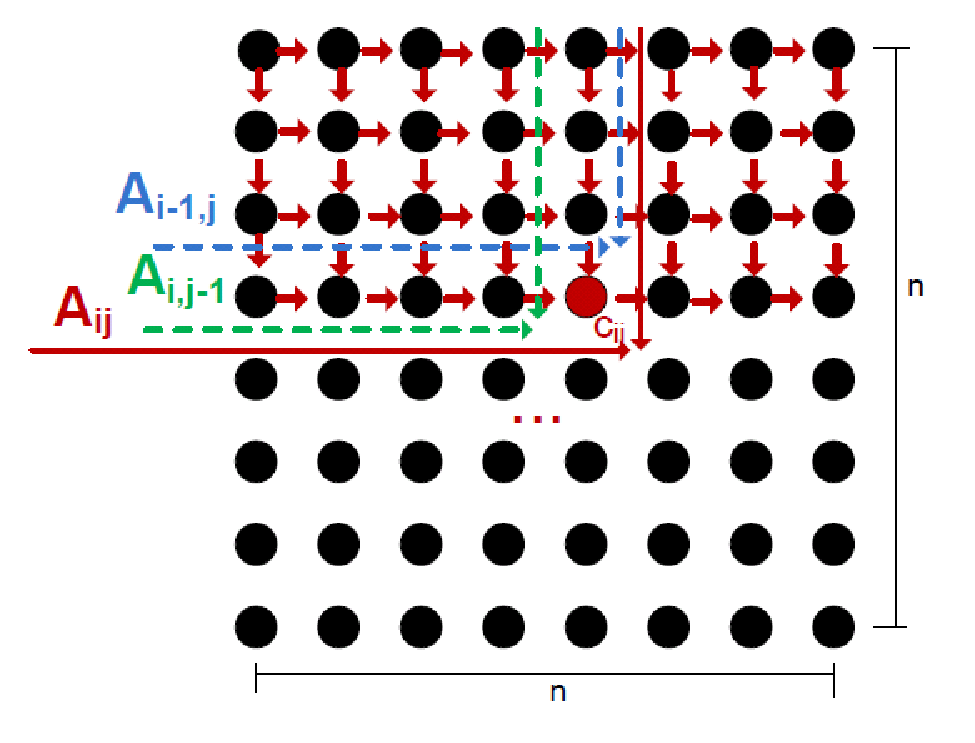
\includegraphics[width=0.4\linewidth]{figtkde/prea}
\label{prec:subfig1}
}
~~\subfloat[Pre-computation of set B]{
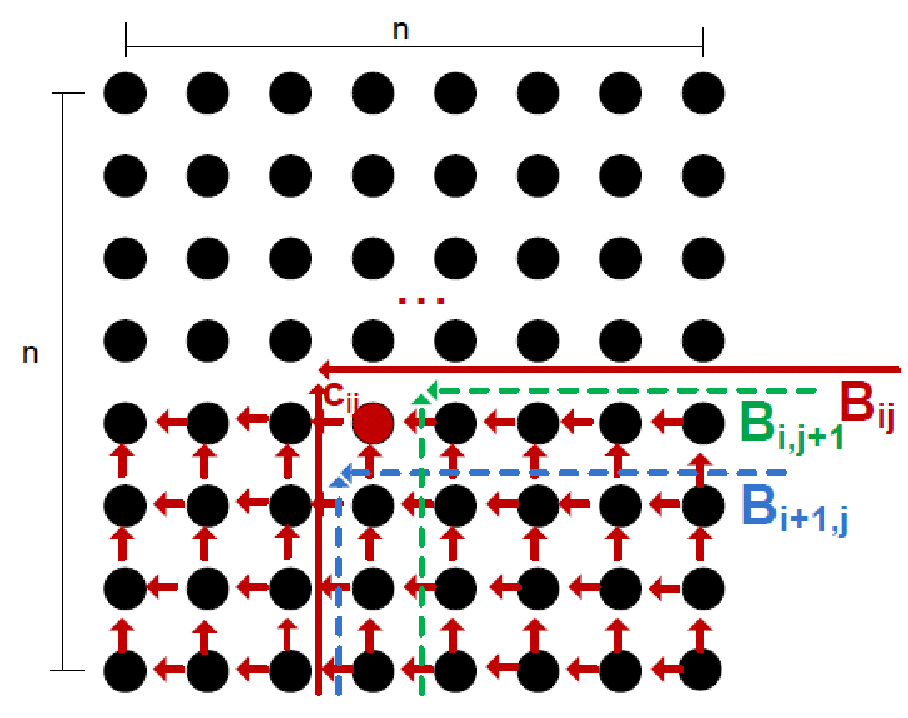
\includegraphics[width=0.4\linewidth]{figtkde/preb}
\label{prec:subfig2}
}\\
~~\subfloat[Pre-computation of set X]{
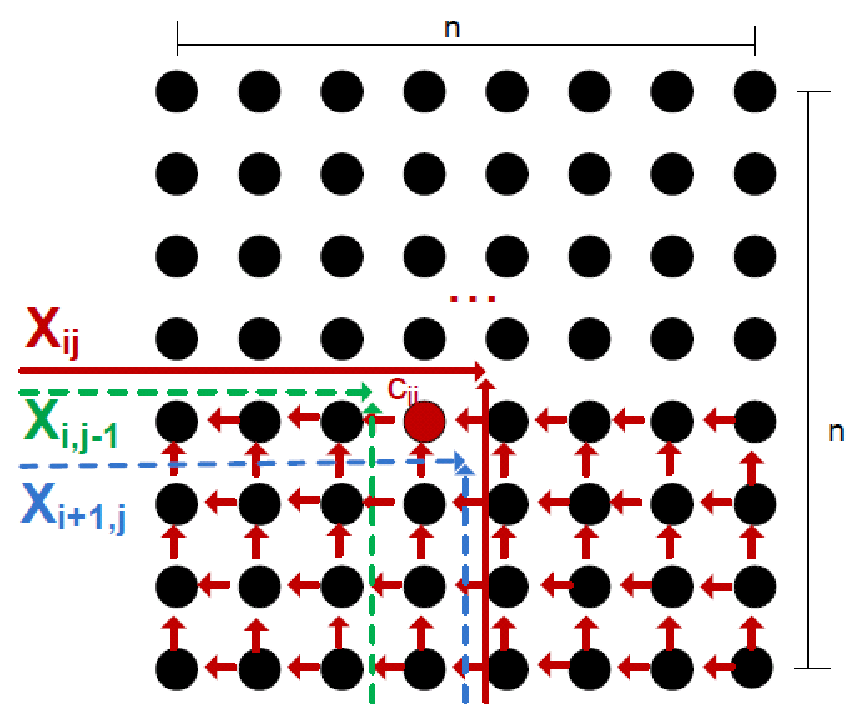
\includegraphics[width=0.4\linewidth]{figtkde/prex}
\label{prec:subfig3}
}
~~\subfloat[Pre-computation of set Y]{
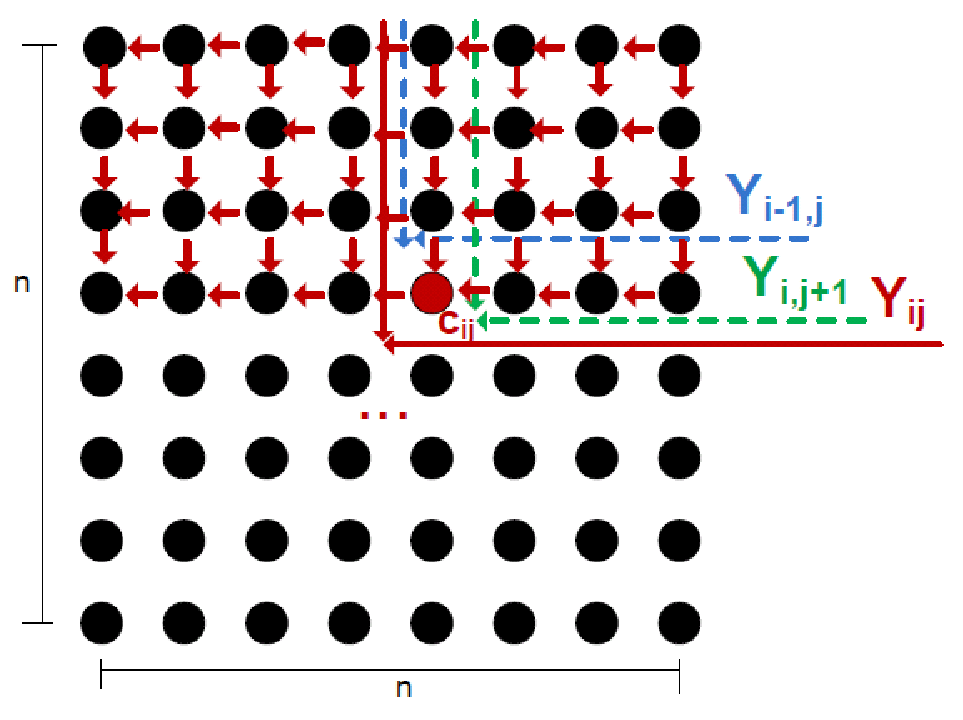
\includegraphics[width=0.4\linewidth]{figtkde/prey}
\label{prec:subfig4}
}
\caption{pre-computation of set A, B, X and Y}\label{prec}
\end{figure}

Due to the high dependency among rows and columns, pre-computing is hard to parallelise and the computation is very fast on a CPU. In our work, the pre-computation of set $A, B, X, Y$ is done on a CPU.


\begin{algorithm}[t!]\small
\label{pre1}
\caption{Inclusive/Exclusive Pre-computation for Set A}\label{pre1}
Input: data grid (G) \\
Output: accumulated counts $A(i,j)$\\
------------------------------------------------------------------ \\
\begin{algorithmic}[1]
\STATE //Initialize first element $A(0,0)$
\STATE {\textit { $A(0,0)$\(\leftarrow\)$G(0,0)$}}
\STATE //accumulation of remaining elements in first row
\FOR{\textit  j\(\leftarrow\)1 to \textit{n}}
\STATE{\textit { $A(0,j)$ \(\leftarrow\) $G(0,j)$ +$A(0,j-1)$}}
\ENDFOR
\STATE //accumulation of remaining elements in first column
\FOR{\textit  i\(\leftarrow\)1 to \textit{n}}
\STATE  {\textit {$A(i,0)$\(\leftarrow\)$G(i,0)$ + $A(i-1,0)$}}
\ENDFOR
\STATE //accumulation of all the elements in remaining rows and columns
\FOR{\textit  k\(\leftarrow\)1 to \textit{n}}
\FOR{\textit  i\(\leftarrow\)k to \textit{n}}
\STATE  {\textit { $A(i,k)$\(\leftarrow\) $G(i,n+k)+A(i-1,k)+A(i,k-1)-A(i-1,k-1)$}}
\ENDFOR
\FOR{\textit  j\(\leftarrow\)k to \textit{n}}
\STATE  {\textit { $A(k,j)$\(\leftarrow\) $G(k,n+j)+A(k,j-1)+ A(k-1,j)-A(k-1,j-1)$}}
\ENDFOR
\ENDFOR
\end{algorithmic}
\end{algorithm}



\section {Range Mapping Scheme} \label{RMS}
The main problem we study in this section is how to parallelize the enumeration of all rectangular regions (R) in a spatial grid (G).

Firstly, we propose a range mapping scheme to transform all of the pairwise intervals between data points from non-consecutive space to consecutive space for $n$ data points in one dimension. Then we extend this scheme to two dimensional spatial grid and multi-dimensional grid. After transformation, the consecutive space enables the overall intervals/regions to be partitioned into equal portions and distributed onto each ``parallel computing unit'' (PCU).

\subsection {One Dimensional Point Set}
In one dimension, axis oriented rectangles become intervals that have both endpoints in the unit interval and we assume $X=\{x_0,x_1,x_2,...,x_n\}$ is a set of $(n+1)$ distinct points.

To enumerate all of the pairwise points between these points, the interval set is defined as:  $ \mathbb{R}=\{I(i,j)|{0 \le {i} \le n,i \le {j} \le n} \}$ in 2D coordinate system. We assume each interval $I(i,j)$ is corresponding to a point $(i,j)$ in 2D coordinate system. Regions are formed by these points.
\vspace{5pt}
\begin{definition}
$\textbf {Interval I(i,j):}$ An interval $I(i,j)\in \mathbb{R}$ represents the distance from start point $x_i$ to end point $x_{(j+1)}$. For example, to denote the interval from the start point $x_0$ to the end point $x_1$, we define it as $I(0,0)$. $I(0,1)$ denotes the interval from the start point $x_0$ to the end point $x_2$, etc.
\end{definition}

\vspace{5pt}

\begin{definition}
$\textbf {Closed Bounded Region }$
$CBR(i,j) \rightarrow CBR(i_k,j_k) ...\rightarrow CBR(i_n,j_n):$ This closed bounded region represents the closed area from point $(i,j)$ to $(i_k,j_k)$ ,..., at last to end point $(i_n,j_n)$.
\end{definition}

\vspace{5pt}

\begin{lemma}$\textbf {Range Mapping-{1D}:}$ In one dimensional space, there has a bijective function $f_{1d}:I(i,j)\rightarrow I(i',j')$ , where each interval $I(i,j)\in$ $\{{0 \le {i} \le n,i \le {j} \le n} \}$ is mapped to by exactly one interval $I(i',j')\in$ $\{{0 \le  {i'} \textless {\frac {n} {2}},0 \le {j'} \le n}\}$.
\end{lemma}

\begin{proof}
The cardinality of the intervals in one dimensional point set X is $|{R}|={\frac{n \cdot (n+1)}{2}}$. To visualize, each different interval $(i,j)$ from set X is plotted out in Figure~\ref{trans:subfig1} in 2D coordinate system. It is clearly to be seen that this domain has triangular shape and the total amount of intervals can be split into the product of ${\frac{n} {2}}$ and $(n+1)$. It has the exactly same amount of all the points within the rectangular space of $[{\frac{n} {2}},n+1]$. Therefore, there exists a one-to-one onto mapping of the data points in the triangular shaped space to the data points in the rectangular shaped space.

Figure~\ref{trans:subfig2} shows the original point (interval) space and the transformed point (interval) space. Both of them consist of the same number of points, which creates the same amount of intervals. The implementations of brute-force approach and workable parallel approach from $(i,j)$ to $(i,j')$ are shown in the Algorithm~\ref{RM1} and ~\ref{RM2}. The detailed transform approach is given in the following part.


\begin{figure}[h]
\centering
\subfloat[]{
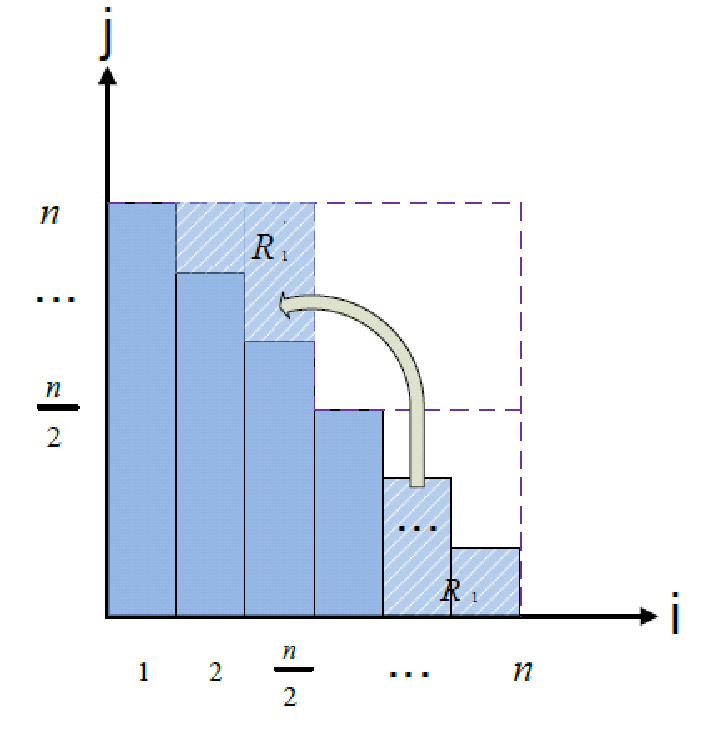
\includegraphics[width=0.45\linewidth]{figtkde/trans1d}
\label{trans:subfig1}
}
~~\subfloat[]{
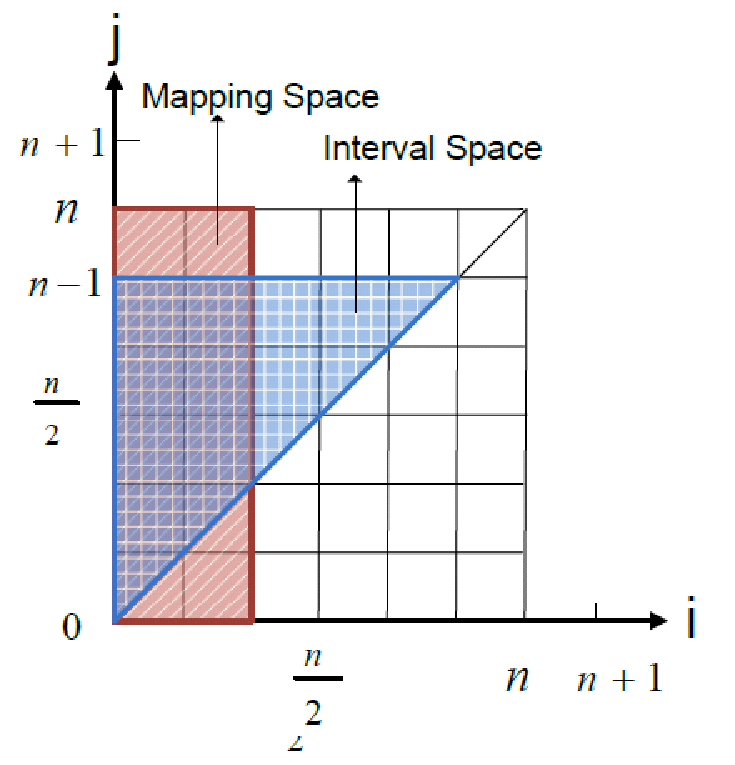
\includegraphics[width=0.45\linewidth]{figtkde/mappingorg}
\label{trans:subfig2}
}
\caption{1-d Interval Transformation from $[n,n]$ to $[(n+1)/2,n]$}\label{modelBF}
\end{figure}

\begin{algorithm}[t!]\small
\label{al}
\caption{Brute-force Range Mapping in 1-d array}\label{RM1}
Input:  n data points \\
Output: LRT of all the intervals among n points\\
------------------------------------------------------------------ \\
\begin{algorithmic}[1]
\FOR{\textit i \(\leftarrow\)0 to \textit{n-1}}
\FOR{\textit j \(\leftarrow\)i to \textit{n-1}}
\STATE \textit {LRT computation for interval {i,j}}
\ENDFOR
\ENDFOR
\end{algorithmic}
\end{algorithm}

\begin{algorithm}[t!]\small
\label{al}
\caption{ Parallel Interval Enumeration in 1-d array}\label{RM2}
Input:  n data points \\
Output: LRT of all the intervals in parallel\\
------------------------------------------------------------------ \\
\begin{algorithmic}[1]
\STATE \textit For each i $\in \{0,..,{\frac{n}{2}-1}\}$,
\STATE //The interval (i,j) is determined through two independent loops
\STATE //loop 1
\FOR{\textit j \(\leftarrow\)i to \textit{n-1}}
\STATE \textit {LRT computation for interval (i,j)}
\ENDFOR
\STATE //loop 2
\FOR{\textit j \(\leftarrow\){n-i} to \textit{n-1}}
\STATE \textit {LRT computation for interval (i,j)}
\ENDFOR
\end{algorithmic}
\end{algorithm}
\end{proof}

Lemma 1 is applicable only when the number of the points in set X is even, to make it more applicable, we extend it workable for set X having even/odd number of points.

\begin{lemma}{$ \textbf {Range Mapping-{EO}:}$ }
There has a injective function $f_{eo}:(i,j)\rightarrow (i',j')$ , where each interval $I(i,j)\in$ $\{{0 \le {i} \le n,i \le {j} \le n} \}$ is mapped to at most one interval $I(i',j')\in$ $\{{0 \le {i'} \le \lfloor {\frac {n+1} {2}}\rfloor ,0 \le {j'} \le n+1}\}$.

\end{lemma}
\begin{proof}
We know the cardinality of the intervals in one dimensional point set X is $|{R}|={\frac{n \cdot (n+1)}{2}}$. This is the product of $(n+1)$ and $\frac{n} {2}$. Dependent on $n$, the number of points in rectangular shaped space generated by the second part $\frac{n} {2}$ together with $(n+1)$, will be less than or equal to the total number of points required by triangular shaped space. If we extend $\frac{n} {2} $ to $\frac{(n+1)} {2} $ ($\frac{n} {2} \le \lfloor {\frac {n+1} {2}}\rfloor$), each interval included in the triangular shaped space is exactly mapped to one point in the transformed rectangular space.


Figure~\ref{even:subfig1} and Figure~\ref{odd:subfig1} show the solutions and implementation is shown in Algorithm~\ref{RM}. There are points $\{x_0,x_1,x_2,...,x_n\}$, to transform the rectangular range space to the triangular space, two scenarios and corresponding transformation steps are considered:

\noindent $ \textbf {Scenario I:}$ When there are even number of intervals (i.e. $(n+1)$ $mod $$2 \equiv 0$ ), the rectangular shaped space and triangular shaped space are shown in Figure~\ref{even:subfig1} and bounded by: \\$ {CBR_{rec}=CBR_{(0,0)} \rightarrow CBR_{(\frac{n} {2}-1,0)} \rightarrow CBR_{(\frac{n} {2}-1,n)}}$\\ $\rightarrow CBR_{(0,n)}$
and
\\${CBR_{tri}=CBR(0,0) \rightarrow CBR_{(n-1,n-1)} \rightarrow CBR_{(0,n-1)}}$.\\
To perform mapping, two lines $i=j$ and $i+j=n$ divide $CBR_{rec}$ into three parts: $(1)  T_1=\{(i,j)|(i+j)\ge n\}$, $(2) T_2=\{(i,j)|j\textless  i\}$, $(3) T_3=\overline{T1\cap T2}$. The steps are:

\begin{itemize}
\renewcommand{\labelitemi}{$\bullet$}
\item   $\forall (i,j)\in T_2$ are shifted upwards by $|i|$ into $CBR_{tri}$. ${R_1}'$ are transformed to ${R_1}$ in the figure.
\item  $\forall (i,j)\in T_1$ are shifted downwards by $|j-n+1|$ and shifted rightwards in a by $|2(\frac{(n)} {2}-i)-1|$. ${R_2}'$ is transformed to $R_2$ in the figure.
\item  $\forall (i,j)\in T_3$ are shifted upwards by $|i|$ until reaching line $i+j=n$.
\end {itemize}

\noindent $ \textbf {Scenario II:}$ When there are odd number of intervals (i.e. $(n+1)$ $mod $$2 \neq 0$), the rectangular and triangular shaped space are shown in Figure~\ref{odd:subfig1} and bounded by:
  \\$ {CBR_{rec}=CBR_{(0,0)} \rightarrow CBR_{(\frac{(n-1)} {2},0)} \rightarrow CBR_{(\frac{(n-1)} {2},n)}}$\\ $\rightarrow CBR_{(0,n)}$
and
\\${CBR_{tri}=CBR(0,0) \rightarrow CBR_{(n-1,n-1)} \rightarrow CBR_{(0,n-1)}}$.\\The steps are almost same as the steps for transforming even number of intervals. The only difference is the intervals in the rectangular space of $ {CBR_{(0,0)} \rightarrow CBR_{(\frac{(n-1)} {2}-1,0)} \rightarrow CBR_{(\frac{(n-1)} {2}-1,n)}}$\\ $\rightarrow CBR_{(0,n)}$ are transformed. The intervals $(i,j)\in CBR_{tri} $ when $j=(n+1)/2$ are remained at their positions.


\end{proof}

\begin{algorithm}[t!]\small
\label{RM}
\caption{ Parallel Range Mapping in 1-d array}\label{RM}
Input:  n data points \\
Output: mapping all the intervals from rectangular to triangular space\\
------------------------------------------------------------------ \\
\begin{algorithmic}[1]
\STATE //The interval (i',j') in rectangular space is transformed to interval (i,j) in triangular space
\FOR{\textit i' \(\leftarrow\)0 to \textit{(n+1)/2}}
\FOR{\textit j' \(\leftarrow\)0 to \textit{n}}
\IF{$j'\textless (n-i')$ }
\STATE{\textit i\(\leftarrow\)i'}
\STATE{\textit j\(\leftarrow\)(i'+j')}
\ELSE
\IF{$2(i'+1)\textless (n+1)$ }
\STATE {\textit i\(\leftarrow\)(n-i'+1)}
\STATE {\textit j\(\leftarrow\)(n-j'+i)}

\ENDIF
\ENDIF
\STATE \textit {LRT computation for interval (i,j)}
\ENDFOR
\ENDFOR
\end{algorithmic}
\end{algorithm}


\begin{figure}[h]
\centering
\subfloat[Solution when Grid size n is even number ]{
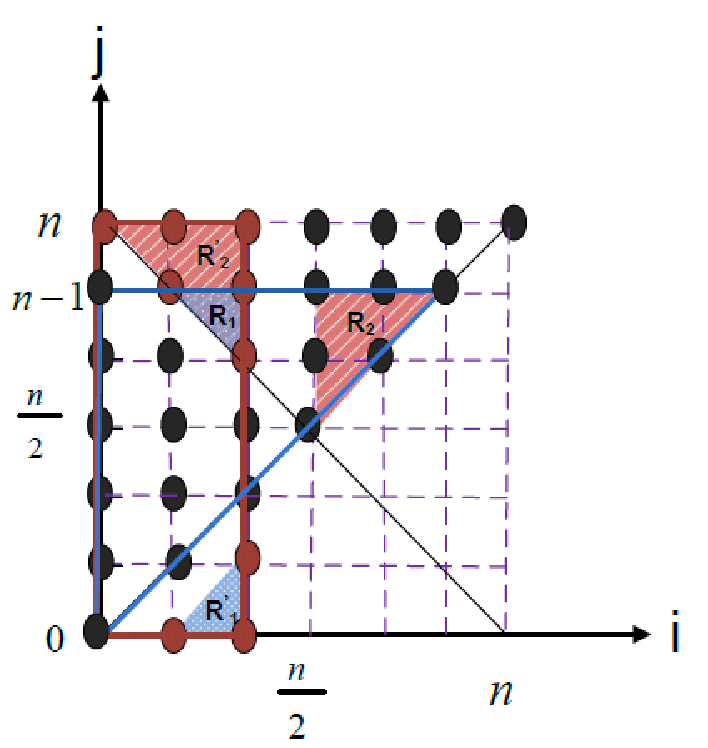
\includegraphics[width=0.45\linewidth]{figtkde/eventransform}
\label{even:subfig1}
}
~~\subfloat[Solution when Grid size n is odd number ]{
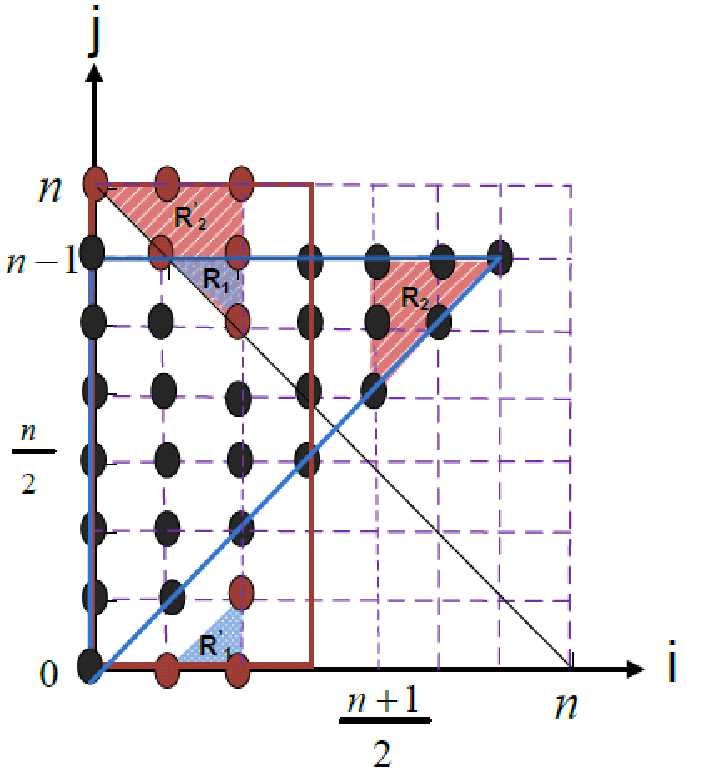
\includegraphics[width=0.45\linewidth]{figtkde/oddtransform}
\label{odd:subfig1}
}
\caption{1-d Interval Transformation from $[n,n]$ to $[\lfloor (n+1)/2 \rfloor,n+1]$}\label{modelBF}
\end{figure}

$\noindent \textit {Example:}$ To illustrate the transformation, Figure~\ref{example:subfig1} and ~\ref{example:subfig2} show small examples on how to transform the intervals when having data points $\{x_0,x_1,x_2,x_3,x_4\}$ and $\{x_0,x_1,x_2,x_3,x_4,x_5\}$ respectively. For data point $(i,j)\in \{x_0,x_1,x_2,x_3,x_4\}$, the total intervals is $10$. By plotting out all of them in Figure~\ref{example:subfig1}, the triangular shaped space is bounded by $(0,0)\rightarrow(3,3)\rightarrow (0,3)$ and there are exactly $10$ points in total. The rectangular shaped space is bounded by $(0,0)\rightarrow(1,0)\rightarrow (1,4)\rightarrow (0,4)$ and total number of points is exactly $10$. Similarly, for data point $(i,j)\in \{x_0,x_1,x_2,x_3,x_4,x_5\}$,  the triangular shaped space is bounded by $(0,0)\rightarrow(3,3)\rightarrow (0,3)$ and total number of points is . The rectangular shaped space is bounded by $(0,0)\rightarrow(1,0)\rightarrow (1,4)\rightarrow (0,4)$ and total number of points is exactly $10$. Table~\ref{maptable} shows the transformations.
\begin{figure}[h]
\centering
\subfloat[ Grid size n =4 ]{
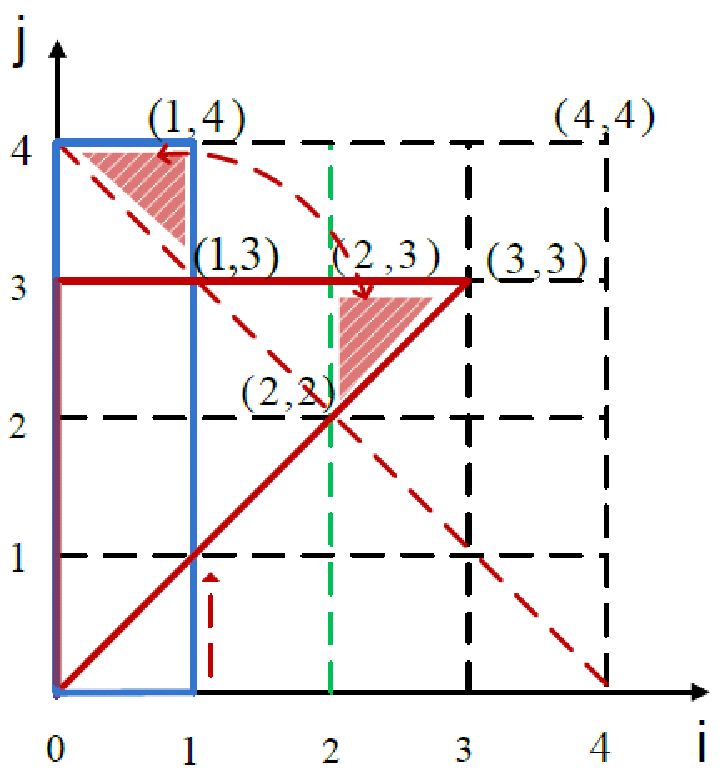
\includegraphics[width=0.45\linewidth]{figtkde/exampleven}
\label{example:subfig1}
}
~~\subfloat[Grid size n =5 ]{
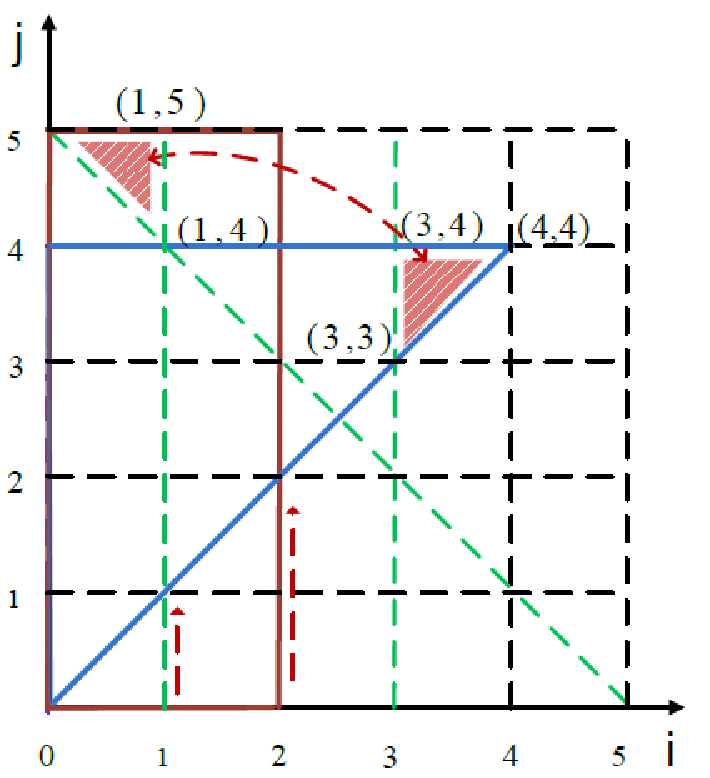
\includegraphics[width=0.45\linewidth]{figtkde/exampleodd}
\label{example:subfig2}
}
\caption{Example: 1-d Interval Transformation}\label{example}
\end{figure}


\begin{table}[!ht]\small
  \centering \small
  \subfloat[Grid (4,4)\label{maptable1}]{
    \centering \small
     \begin{tabular}{|c|c|}
	\hline
    $from (i,j)$  & $to (i',j')$\\
    	\hline
    (0,0)  & (0,0)  \\
    \hline
    (0,1)  & (0,1) \\
    \hline
        (0,2)  & (0,2)  \\
    \hline
    (0,3)  & (0,3) \\
    \hline
     (0,4)  & (3,3) \\
    \hline
            (1,4)  & (2,2)  \\
    \hline
    (1,3)  & (2,3) \\
    \hline
           (1,0)  & (1,1)  \\
    \hline
    (1,1)  & (1,2) \\
    \hline
     (1,2)  & (1,3) \\
    \hline

\end{tabular}
  }
  \subfloat[Grid (5, 5)\label{maptable2}]{
    \centering \small
   \begin{tabular}{|c|c|}
	\hline
    $from (i,j) $  &  $to (i',j')$ \\
       	\hline
    (0,0)  & (0,0)  \\
    \hline
    (0,1)  & (0,1) \\
    \hline
        (0,2)  & (0,2)  \\
    \hline
    (0,3)  & (0,3) \\
        \hline
    (0,4)  & (0,4) \\
    \hline
     (0,5)  & (4,4) \\
    \hline
            (1,0)  & (1,1)  \\
    \hline
    (1,1)  & (1,2) \\
    \hline
    (1,2)  & (1,3) \\
    \hline
     (1,3)  & (1,4) \\
    \hline
            (1,4)  & (3,4)  \\
    \hline
    (1,5)  & (3,3) \\
    \hline
    (2,0)  & (2,2) \\
    \hline
     (2,1)  & (2,3) \\
    \hline
            (2,3)  & (2,4)  \\
    \hline
\end{tabular}
  }
  \caption{Example: Interval Transformation for even/odd number of points }\label{maptable}
\end{table}

\begin{comment}
\begin{table}[!ht]\small
  \centering \small
  \subfloat[Grid (4,4)\label{maptable1}]{
    \centering \small
     \begin{tabular}{|c|c|}
	\hline
    $from $  & to \\
\end{tabular}
  }\\
  \subfloat[Grid (5,5)\label{maptable2}]{
    \centering \small
   \begin{tabular}{|c|c|c|c|c|c|c|c|c|}
	\hline
From  &(0,0)& (0,1)& (0,2)& (0,3)& (0,4)& (0,5)  &  (1,0)& (1,1) \\
\hline
To & (0,0)& (0,1)& (0,2)& (0,3)& (0,4)& (4,4) & (1,1)& (1,2) \\
\hline
From  &(1,2) & (1,3)& (1,4)& (1,5)& (2,0)& (2,1)  &  (2,3)& (1,1) \\
\hline
To & (1,3) & (1,4)& (3,4)& (3,3)& (2,2)& (2,3) & (2,4)& (1,2) \\
\hline
\end{tabular}
  }
  \caption{Example: Interval Transformation for even/odd number of points }\label{maptable}
\end{table}

\end{comment}
\subsection {Two Dimensional Region Set}
\begin{lemma}$ \textbf {Range Mapping-{2D}:}$
In two dimensional grid $(m,n)$, there has a injective function $f_{2d}:R(i_1,j_1,i_2,j_2)\rightarrow R(i'_1,j'_1,i'_2,j'_2)$ is mapped to at most one region:\\
$\{({i_1}',{j_1}',{i_2}',{j_2}')|{0 \le {{i_1}'} \le {\lfloor \frac {m+1} {2}\rfloor},0 \le {{j_1}'} \le m+1},\\{0 \le {{i_2}'} \le {\lfloor \frac {n+1} {2}\rfloor},0 \le {{j_2}'} \le n+1}\}$.
\end{lemma}
\begin{proof}
We know that a region is bounded by two vertical lines $(x=i_1, x=i_2)$ and two horizontal lines $(y=j_1, y=j_2)$. The coordinates of $x$ and $y$ are independent of each other for defining a region. That means $(i_1,i_2)$ is independent to $(j_1, j_2)$. From above, there has injective function to transform each interval in one dimension. Therefore, all rectangular regions in grid $(m,n)$ can be transformed to 2D rectangular region with $\{({\lfloor \frac {m+1} {2}\rfloor},m+1),({\lfloor \frac {n+1} {2}\rfloor},n+1)\}$.
\end{proof}
\subsection {Multi-Dimensional Point Set}
\begin{lemma}$ \textbf {Range Mapping-{mD}:}$
In multi-dimension grid $(n_1,n_2,...,n_m)$, there has a injective function $f_{md}:R(i_1,j_1,i_2,j_2,...,i_m,j_m)\rightarrow R(i'_1,j'_1,i'_2,j'_2,...,i'_m,j'_m)$ is mapped to by at most one region:\\ $\{({i_1}',{j_1}',{i_2}',{j_2}',...,{i_m}',{j_m}')\\|{0 \le {{i_1}'} \le {\lfloor \frac {{n_1}+1} {2}\rfloor},0 \le {{j_1}'} \le {n_1}+1},\\{0 \le {{i_2}'} \le {\lfloor \frac {{n_2}+1} {2}\rfloor},0 \le {{j_2}'} \le {n_2}+1},...,\\{0 \le {{i_m}'} \le {\lfloor \frac {{n_m}+1} {2}\rfloor},0 \le {{j_m}'} \le {n_m}+1}\}$.
\end{lemma}

\section{ Kbest Reduction Scheme}\label{KBEST}
To find top-k\footnote{We use top-k and kbest exchangeably.} anomalous rectangular regions, a heap with maximium size of k is built from each ``parallel computing unit'' (PCU). A further reduction strategy is applied on these k heaps to get final kbest regions.

A LRT value set $s={s_1,s_2, .., s_i,...,s_n}$ is generated from $n$ rectangular regions set $\mathbb{R}$. $\{R\}$ is divided into $t$ equal portions: ${p_1,p_2,..,p_i,...,p_t}$, where $1\le t\le n$. Each portion is processed in parallel and a $kbest$ result with heap structure is generated correspondingly. The $kbest$ result from each portion is $p_{1_k},p_{2_k},...,p_{i_k},..p_{t_k}$.\\ We denote the process of finding $kbest$ using heap sort as $h()$. We also denote the $kbest$ result from original data grid is $\{s_{r0},s_{r1},...,s_{rk}\}$. And the $kbest$ value from each parallel portion $p_i$ is $\{s_{i0},s_{i1},...,s_{ik}\}$. And we assume the $kbest$ value are in ascending order. For example, $s_{r0}\le s_{r1},...,\le s_{rk}$, $s_{i0}\le s_{i1},...,\le s_{ik}$.
\begin{lemma}{\bf $KBestReduction:$} The $kbest$ LRT values from the value set ${s}$ is equal to the $kbest$ values obtained by performing $kbest$ reduction from each parallel portion:
$h(p_1\cup p_2\cup ...\cup p_i \cup...\cup p_n)=h(h(p_1)\cup h(p_2)\cup ...\cup h(p_n))$.
\end{lemma}
We give proof by contradiction:
\begin{enumerate}[(a)]
\item $\forall x\in h(p_1\cup p_2\cup ...\cup p_i \cup...\cup p_n)$$\rightarrow x\in (h(p_1)\cup h(p_2)\cup ...\cup h(p_n))$$\rightarrow x\in h(h(p_1)\cup h(p_2)\cup ...\cup h(p_n))$. \\$\because $ Total number of $kbest$ values of $|(h(p_1)\cup h(p_2)\cup ...\cup h(p_n)|\ge k$. \\
     And $x \notin h(p_1)\cup h(p_2)\cup ...\cup h(p_n)$ $\rightarrow x \notin h(p_1\cup p_2\cup ...\cup p_i \cup...\cup p_n)$.\\ Furthermore, since $x$ is one of the topk value from all the results, therefore, $x\in h((h(p_1)\cup h(p_2)\cup ...\cup h(p_n)))$
\item $\forall x\in h(h(p_1)\cup h(p_2)\cup ...\cup h(p_n)) $$\rightarrow x\in h(p_1)\cup h(p_2)\cup ...\cup h(p_n)$$\rightarrow x\in h(p_1\cup p_2\cup ...\cup p_i \cup...\cup p_n)$\\
    $\because $ $h(h(p_1)\cup h(p_2)\cup ...\cup h(p_n))\subseteq h(p_1)\cup h(p_2)\cup ...\cup h(p_n) \subseteq h(p_1\cup p_2\cup ...\cup p_i \cup...\cup p_n)$
\end{enumerate}

So the $kbest$ from the whole value set $s$ is same as the reduction from the $kbest$ results from each processes. We implemented $minheap$ and $maxheap$ to store the $kbest$ results for each parallel threads/process. Please see algorithm

\section {Implementations on Parallel and Distributed Architecture }\label{IMPDA}
From the above discussion of 2D range mapping scheme, the total rectangular regions can be transformed from triangular shaped space to rectangular shaped space. This mapping have a contiguous space without gap to enable the workload perfectly partitioned into same amount for multi-core, pc-cluster and GPGPU architectures. The effects of coarse-grained and fine-grained parallelism are shown in Figure~\ref{scheme:rm1} and ~\ref{scheme:rm2}.

 \begin{figure}[h]
\centering
\subfloat[Workload Balance of Rectangular Range Mapping Scheme]{
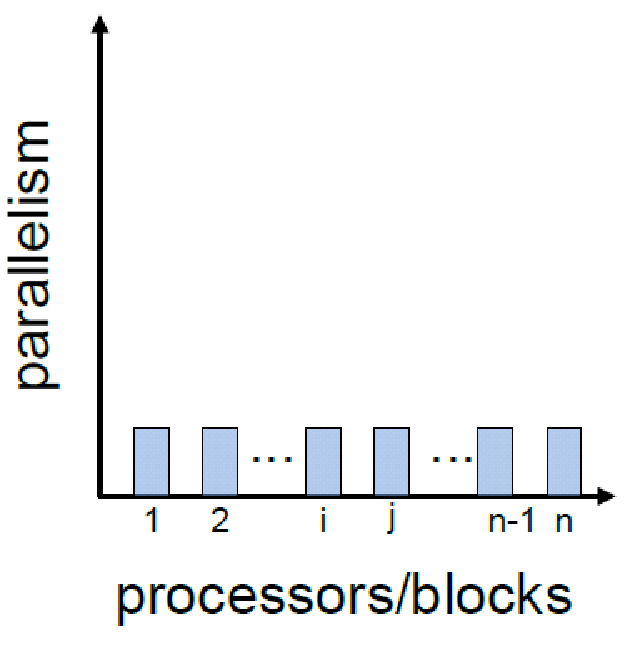
\includegraphics[width=0.45\linewidth]{figtkde/rangemapping1}
\label{scheme:rm1}
}
~~\subfloat[Workload Imbalance of Triangular Range Scheme ]{
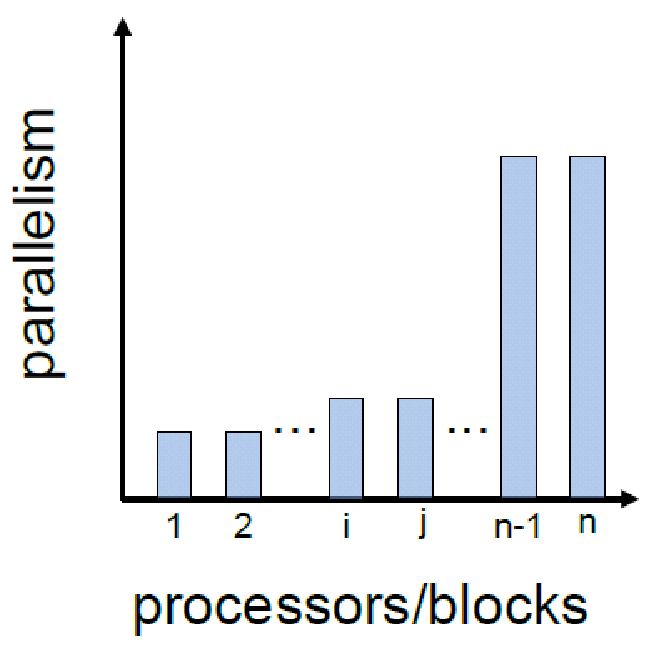
\includegraphics[width=0.45\linewidth]{figtkde/rangemapping2}
\label{scheme:rm2}
}
\caption{The parallelism comparison between rectangular and triangular range mapping scheme applied to enumeration of regions }\label{scheme}
\end{figure}


We implemented the range mapping scheme on different parallel and distributed architectures: Multi-core, GPGPU and EC2 Cloud Cluster.

\subsection{Naive Approach}
Firstly, we introduce the naive approach of LRT computation on a two-dimensional grid $(n,n)$.
In spatial anomaly detection, all the contiguous and rectangular areas are searched and LRT computation is performed over each of them. The regions within top-k LRT statistic values are treated as potential outliers. The implementation is shown in algorithm~\ref{naive}. We can see the computation complexity of brute-force searching is $\bigo(n^4)$ and the computation complexity of single LRT for a region $R$ is $\bigo(cn^2)$. Therefore, the total computation complexity of naive approach in 1EXP family is $\bigo(cn^6)$.

\begin{algorithm}[t!]\small
\label{algobr1}
\caption{Naive top-k LRT search}\label{naive}
Input: data grid (G(n,n)), k\\
Output: top k anomalous regions\\
------------------------------------------------------------------ \\
\begin{algorithmic}[1]
\STATE //Search each rectangle R (x1,y1,x2,y2) in G (n,n)
\FOR{\textit x1 \(\leftarrow\)0 to \textit{n}}
\FOR{\textit y1 \(\leftarrow\)0 to \textit{n}}
\FOR{\textit x2 \(\leftarrow\)x1 to \textit{n}}
\FOR{\textit y2 \(\leftarrow\)y1 to \textit{n}}
\STATE {\textit {score\(\leftarrow\)lrt(x1,y1,x2,y2)}}
\ENDFOR
\ENDFOR
\ENDFOR
\ENDFOR
\STATE {\textit {Sorting the scores and return top-k regions R }}
\end{algorithmic}
\end{algorithm}

\subsection{Inclusive/Exclusive Approach}
Inclusive/Exclusive scheme in section 3 is applied on the whole spatial grid (G) to generate four pre-computed data set. For any given region $R$, retrieving the intermediate statistic value is $\bigo(1)$ time. The overall enumeration cost is reduced in a sequential version. The kbest heap structure is built to keep global top-k regions. The implementation is shown in algorithm~\ref{Inex}.
\begin{algorithm}[t!]\small
\label{algobr1}
\caption{Inclusive/Exclusive top-k LRT search}\label{Inex}
Input: data grid (G(n,n)), k\\
Output: top k anomalous regions\\
------------------------------------------------------------------ \\
\begin{algorithmic}[1]
\STATE //Inclusive/Exclusive pre-computation
\STATE \textit  {prefix\_sums\(\leftarrow\)compute\_prefix\_sums(A,B,X,Y)}
\STATE //Search each rectangle R (x1,y1,x2,y2) in G (n,n)
\FOR{\textit x1 \(\leftarrow\)0 to \textit{n}}
\FOR{\textit y1 \(\leftarrow\)0 to \textit{n}}
\FOR{\textit x2 \(\leftarrow\)x1 to \textit{n}}
\FOR{\textit y2 \(\leftarrow\)y1 to \textit{n}}
\STATE {\textit {intermediate statistics\(\leftarrow\)prefix\_sums(x1,y1,x2,y2)}}
\STATE {\textit {score\(\leftarrow\)lrt(x1,y1,x2,y2,intermediate statistics)}}
\STATE //keep kbest regions
\STATE \textit {kbest \(\leftarrow\)heap(R,G)}
\ENDFOR
\ENDFOR
\ENDFOR
\ENDFOR
\end{algorithmic}
\end{algorithm}

\subsection{Multi-core Approach}
Multi-core computers, computers consisting two or more processors working together on a single integrated circuit, have produced breakthrough performance. They allow faster execution of applications by taking advantage of parallelism, or the ability to work on multiple problems simultaneously. The default mechanism for running parallel programs on multi-core processors is to run a separate process on each core. Threads enable a lighter weight approach than processes. A standardized programming interface called POSIX (Portable Operating System Interface for Unix) was developed to support multiple architecture and provide the capabilities of threads. Implementations adhering to this standard are refereed as Pthreads. Pthreads provide task and data parallelism and flexibility to the programmers.

There are two key advantages associated with LRT computation work on a multi-core architecture with Pthreads. Firstly, for a 1EXP family data grid, LRT computation of each rectangular region is independent. This provides the task parallelism. Secondly, the non-gap ranging mapping scheme clearly enables us to divide the workload to each thread equally, improving scaling.

The implementation of multi-core version is shown in algorithm~\ref{multicorem} and algorithm~\ref{multicorep}. In the main program, each thread is assigned with the same workload and same size of range. It is equal to: total number of regions to be searched divides by the defined number of threads. The range mapping scheme enables each thread to process in a non-gap rectangular range. Otherwise, it is hard to provide each thread same size of range. Each thread performs LRT computation on its own part and keeps $kbest$ regions using $min, max$ heap structure. After all threads finishes computation, the heap function is applied to all the $kbest$ results and get the final $kbest$ regions.

\begin{algorithm}[t!]\small
\caption{LRT implementation on $Multi\-core$ Architecture: Main Part}\label{multicorem}
Input: data grid (G), likelihood function (f)\\
Output: top k anomalous regions\\
------------------------------------------------------------------ \\
\begin{algorithmic}[1]

\STATE //declare threads array
\STATE \textit  {pthread\_t\(\leftarrow\)thread[num\_threads]}
\STATE \textit  {thread\_param \(\leftarrow\)param[num\_threads]}
\STATE // do pre-computation
\STATE \textit  {prefix\_sums\(\leftarrow\)compute\_prefix\_sums()}
\STATE // total workload be partitioned
\STATE \textit  {size\(\leftarrow\) ${((n+1)(n+1))^2/4}$\\}
\STATE // compute the workload of each thread
\STATE \textit  {stride\(\leftarrow\) {size/num\_threads}\\}
\STATE // initialize thread parameters and spawn threads
\FOR{\textit i \(\leftarrow\)0 to \textit{num\_threads}}
\STATE \textit {thread\_param[i].start\(\leftarrow\)start}
\STATE \textit {thread\_param[i].end\(\leftarrow\)start+stride}
\STATE \textit {thread\_param[i].prefix\(\leftarrow\)prefix\_sums}
\STATE \textit {create\_pthread(thread\_param)}
\ENDFOR
\STATE \textit {parallel processing (see the algorithm of parallel part)}
\STATE //get kbest regions
\STATE \textit {kbest \(\leftarrow\)heap(kbest[0,...,num\_threads])}
\end{algorithmic}
\end{algorithm}


\begin{algorithm}[t!]\small
\caption{LRT implementation on Multi-core: Parallel Part}\label{multicorep}
Input: prefix-sum,thread id (i) portion index start, end\\
Output: kbest regions processed by thread i\\
------------------------------------------------------------------ \\
\begin{algorithmic}[1]
 \STATE // thread i process regions from (start,end)
\FOR {\textit {portion index \(\leftarrow\)start to end}}
\STATE \textit {LRT computation for regions obtained from index}
\STATE // keep kbest for current thread i
\STATE \textit {kbest \(\leftarrow\)heap(i)}
\ENDFOR
\end{algorithmic}
\end{algorithm}




\subsection{GPU/Multi-GPU Approach}
The General Purpose Graphic Processing Unit (GPGPU) architecture
allows graphic card to be used as general purpose parallel computing
device.  We briefly describe how the NVIDIA's Compute Unified Device Architecture (\cuda) framework supports massively parallel computing \cite{cuda}. A \cuda program consists of one or more phases that are executed on either the host (\cpu) or the device (\gpu). The host code executed on \cpu exhibits little or no data parallelism and the device code (called kernel) executed on \gpu side exhibits high amount of data parallelism. The kernel uses large number of threads to exploit data parallelism. The \cuda threads are
extremely light weight and require very few clock cycles to be generated and scheduled on the \gpu. The key programming challenge is to map the computation and expressing them onto an abstract model consisting of grids, blocks and threads. The kernel is then executed by a grid of thread blocks. Blocks execute concurrently among multiprocessors while threads in a given block execute concurrently within a single multiprocessor. Only threads within a block can cooperate with each other.

To exploit CUDA for the LRT computation, all of regions are mapped from triangular range shape onto rectangular range shape first and extends to $(n+1)(n+1)/2$ range. The rectangular range is divided into different non-overlap blocks with same size. Each block has a number of threads to process a number of rectangular regions. For fast computation, each block searches all of the rectangular regions which can be fitted into shared memory. Each thread is assigned to compute a subset of rectangle. To avoid transfer all the results back CPU, parallel reduction is performed. Each thread keeps a $kbest$ heap. Furthermore, keeping the total $kbest$ heaps not arbitrary, it might lead  to another kernel for parallel reduction. By defining block number and thread number for different size of data grid, each thread is responsible for varied number of rectangles in different kernel. We did the implementation on single GPGPU and multi-GPGPU and measured the performance.  The implementation of single GPGPU is shows in algorithm ~\ref{gpgpus}. For multi-GPGPU implementation, we divide the whole workload equally to each GPGPU. Final $kbest$ regions are obtained after each device return back all the $kbest$ heaps.

\begin{algorithm}[t!]\small
\label{al}
\caption{ \gpu kernel}\label{gpgpus}
Input: a spatial grid \textit{G(n,n)}, number of blocks \textit{(bx,by)}, number of threads per block \textit{(tx,ty)}\\
Output: top k anomalous regions processed by each thread\\
------------------------------------------------------------------ \\
\begin{algorithmic}[1]
\STATE //total regions to be enumerated
\STATE \textit {total\_workload=$(n(n+1)/2)^2$}
\STATE //compute the workload for each thread
\STATE \textit {tx\_size \(\leftarrow\)$(n(n+1)/2 +bx \cdot tx -1)/(bx\cdot tx)$ }
\STATE \textit {ty\_size \(\leftarrow\)$(n(n+1)/2 +by \cdot ty-1)/(by \cdot ty)$ }
\STATE //LRT computation of each thread
\FOR{\textit i \(\leftarrow\)0 to \textit{tx\_size}}
\FOR{\textit j \(\leftarrow\)0 to \textit{ty\_size}}
\STATE //get region coordinates from range mapping scheme
\STATE \textit { $(x_1,y_1,x_2,y_2)$\(\leftarrow\)reverse\_range\_mapping(i,j)}
\STATE //perform LRT computation on region R
\STATE {\textit{ score\(\leftarrow\)lrt($R(x_1,y_1,x_2,y_2)$)}}
\STATE //keep kbest for current thread
\STATE {\textit{kbest\(\leftarrow\)heap(current thread)}}

\ENDFOR
\ENDFOR
\end{algorithmic}
\end{algorithm}

\subsection{Amazon EC2 Cloud Cluster }
Cloud computing offers a highly scalable infrastructure for high performance computing. Amazon Elastic Compute Cloud (Amazon EC2) enables �compute� in the cloud. It is possible to get a set of computing instances on demand without requiring a lot of maintenance and financial resources a common cluster would need. We present our parallel implementation for cloud computing using MPI. The workload is equally assigned to each process based on our range mapping scheme and each process performs LRT computation on each rectangle and produces $kbest$ regions with heap structure using reduce function. The implementation is shown in algorithm~\ref{mpi}.

\begin{algorithm}[t!]\small
\label{al}
\caption{ MPI main program}\label{mpi}
\textbf{Input:}a spatial grid \textit{G(n,n)}, number of processes \textit{np}, top-k \textit{kbest} \\
\textbf{Output:} top-k anomalous rectangular regions\\
------------------------------------------------------------------ \\
\begin{algorithmic}[1]
\STATE //initialize
\STATE \textit {MPI\_init()}
\STATE //broadcast grid information to all nodes
\STATE \textit {MPI\_Bcast(n,n,g)}
\STATE \textit {total\_workload=$(n(n+1)/2)^2$}
\STATE //compute workload for each process
\STATE \textit{stride\(\leftarrow\)(total\_workload+np-1)/np}
\STATE {\textit{start\(\leftarrow\)$processid\cdot stride$}}
\STATE {\textit{end\(\leftarrow\)$start+stride$}}
\STATE //parallel LRT computation
\STATE {\textit{Rectangle r\(\leftarrow\)compute(g,start,end)}}
\STATE //store kbest results for each process
\STATE {\textit{kbest\(\leftarrow\)heap(r)}}
\STATE // reduce operation
\STATE {\textit{MPI\_reduce(kbest)}}
\STATE //root process
\IF {\textit{$processid==0$}}
\STATE {\textit{kbest\(\leftarrow\)qsort(reduced\_kbest)}}
\ENDIF
\STATE {\textit{MPI\_Finalize()}}
\end{algorithmic}
\end{algorithm}

\section{Experiments and Analysis}\label{EA}

\subsection{Performance Analysis}
We have designed and implemented a set of experiments to show and validate the performance speedup on the above different architectures. The experiments are performed on a Poisson distribution model and a randomly generated anomalous region was introduced
for verification in synthetic data sets. Answers to the following questions were sought:
\begin{itemize}
%\setlength{\parskip}{0pt}
\item What are the performance gains of naive versus Inclusive/Exclusive
 approach?
\item How is the multi-core scaling of the LRT computation on Multi-core architecture?
\item What are the performance gains of GPGPU approaches versus Inclusive/Exclusive approach?
\item How is the MPI scaling of LRT computation on PC-cluster?
\item How is the computation speed of LRT computation for $(n,n)$ grid on these architectures?
\end{itemize}

\subsubsection{Naive vs. Inclusive/Exclusive Implementation}
A naive approach requires $\bigo (n^2)$ computation for a given region. In order to improve the computation efficiency, an Inclusive/Exclusive pre-computation approach is devised, which reduces the 1EXP-LRT computation for each region to $\bigo (1)$. We run the two implementations on an 8-core E5520 Intel server to compare their performance. The data grid varies from $(100,100)$ to $(1000,1000)$. In the Inclusive/Exclusive approach, pre-computed sets take up $\bigo (4n^2)$ space and only the $kbest$ results kept in heap structure at the end, therefore the total space complexity is $\bigo (n^2)$. For a naive approach, the computation result of each region is stored into memory and $kbest$ regions are obtained by sorting all of the results at the end. The total results takes $\bigo(n^4)$ space. Due to large memory space required and long computing, the naive approach was only be able to generate the $kbest$ results from $(100,100)$ to $(300,300)$.

From the results in Figure~\ref{fast:subfig1}, we can see that Inclusive/Exclusive approach has a significant speed-up. The number of rectangles per second processed by Inclusive/Exclusive approach is also plotted for various grid sizes in Figure~\ref{fast:subfig2}, it can be seen the result is almost constant, verifying that our Inclusive/Exclusive pre-computation approach search complexity is $\bigo (1)$.


\begin{figure}[h]
\centering
\subfloat[Running time of Naive vs. Inclusive/Exclusive Approach]{
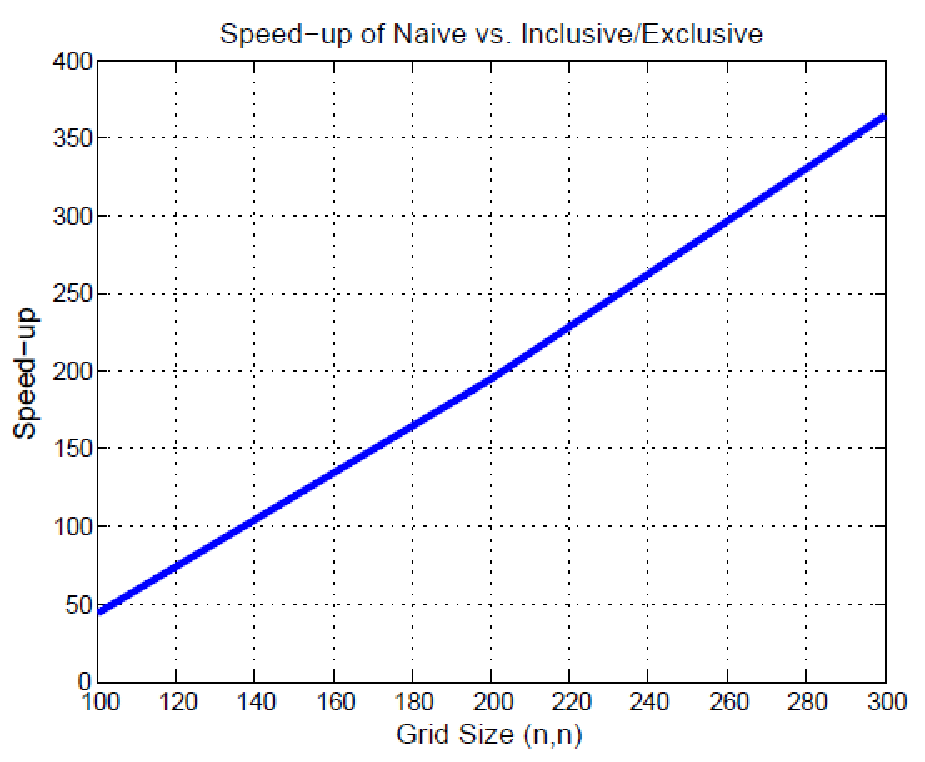
\includegraphics[width=0.75\linewidth]{figtkde/naivespeedup}
\label{fast:subfig1}
}\\
~~\subfloat[No. of Rectangles per second in Inclusive/Exclusive Approach ]{
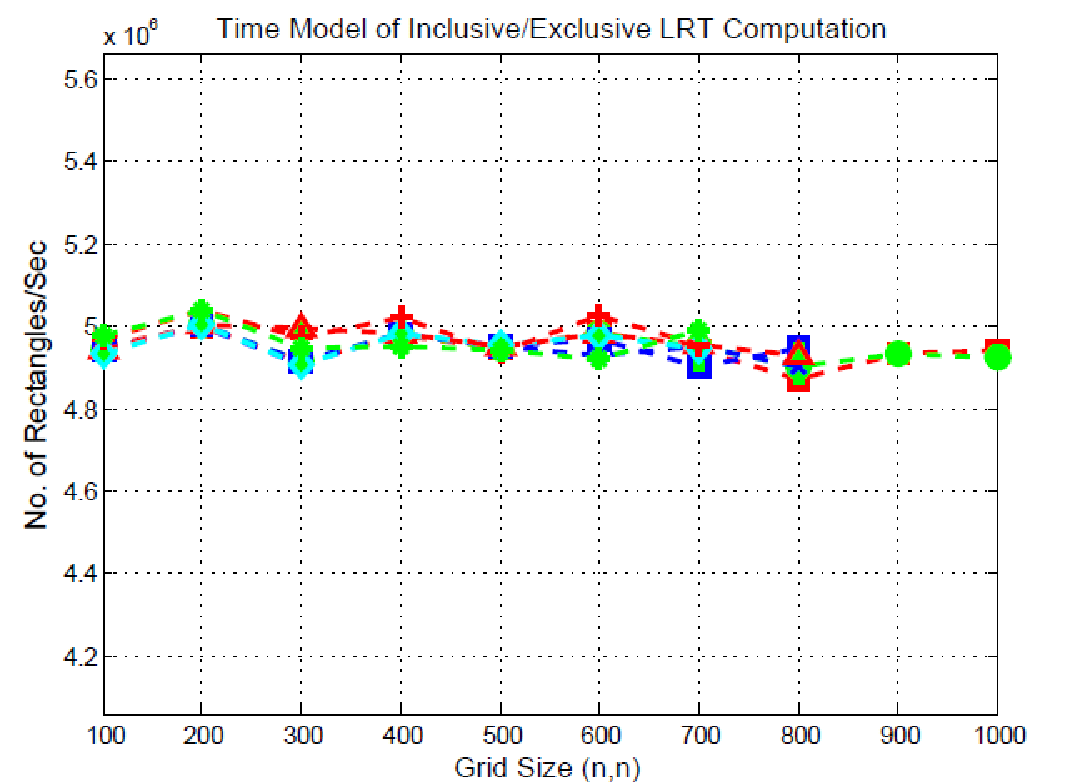
\includegraphics[width=0.8\linewidth]{figtkde/fastspeed}
\label{fast:subfig2}
}
\caption{Naive vs. Inclusive/Exclusive Approach}\label{fast}
\end{figure}
\subsubsection{Multi-core}
 The multi-core experiment is conducted on a 32-core AMD Opteron(tm) Processor 6128 server with 128GB of RAM. We use data grid with size of (1000,1000) to show the performance scaling. Figure~\ref{multicore} shows that the 1EXP-LRT computation scales very well on multi-core architecture.  The speedup increases near-linearly with the increase of number of cores $(no_c)$ and is consistent with the $\bigo(n^4/no_c)$ running time on each core. A speedup of $n$ on $n$ cores is nearly achieved, indicating near perfect scaling (see Figure~\ref{multicore}(a)).

The number of rectangles processed per second is plotted against the number of cores in Figure~\ref{multicore}(b).

\begin{figure}[h]
\centering
\subfloat[Speed-up and Efficiency of Grid (1000,1000) on Multi-core]{
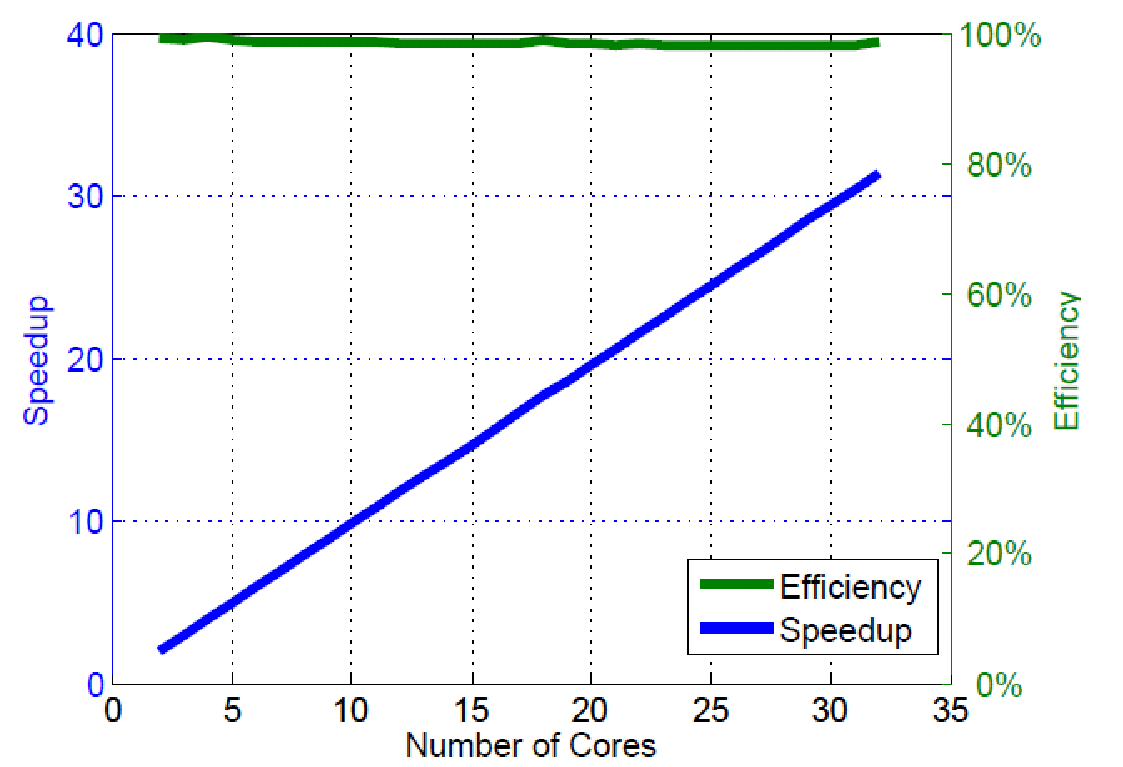
\includegraphics[width=0.9\linewidth]{figtkde/speedup-efficiency}
\label{multicore:multicore1}
}\\
~~\subfloat[The number of rectangles processed per second vs. number of cores on Grid (1000,1000)]{
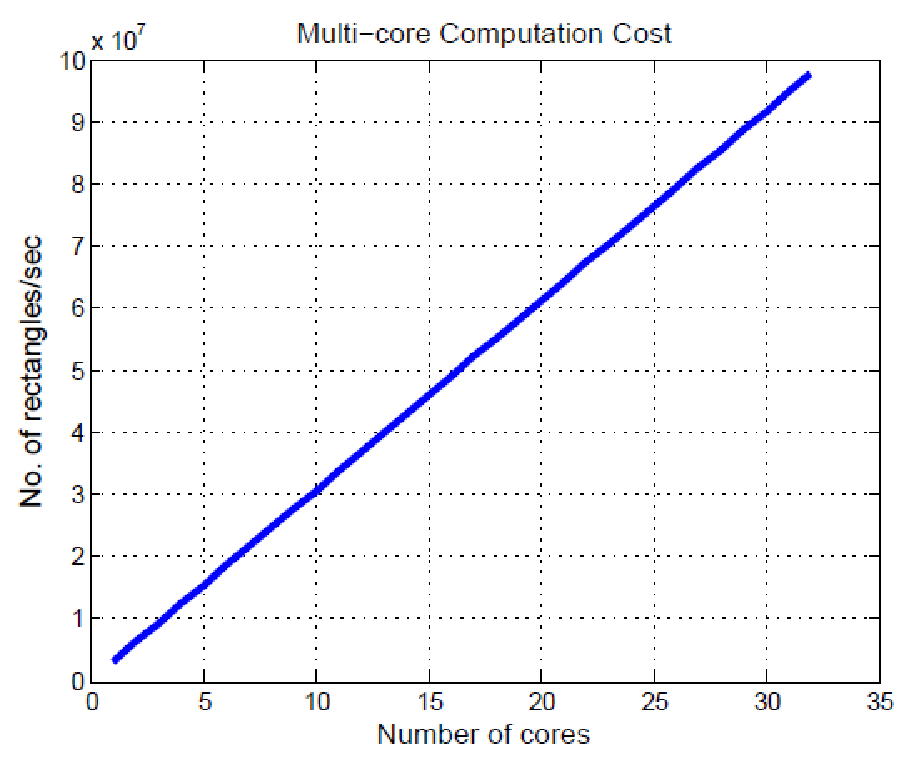
\includegraphics[width=0.8\linewidth]{figtkde/singlerectangle}
\label{multicore2}
}
\caption{Multi-core Evalution}\label{multicore}
\end{figure}

\subsubsection{Multi-GPGPU}
\noindent The experiments were conducted on an 8-core E5520 Intel server that
is equipped with two GPGPU $Tesla$ $C1060$ cards supporting CUDA 4.0.
Each GPGPU card has $4GB$ global memory, $16KB$ shared memory, $240$
cores and $30$ multiprocessors. See Figure~\ref{gpu:subfig1} and ~\ref{gpu:subfig2}.The results show
that LRT computation on two GPGPUs is around 2 times faster than that on one single GPGPU. And the computation
cost of per rectangle is almost constant with the increase
of data grid for single GPGPU and two GPGPUs.

\begin{figure}[h]
\centering
\subfloat[]{
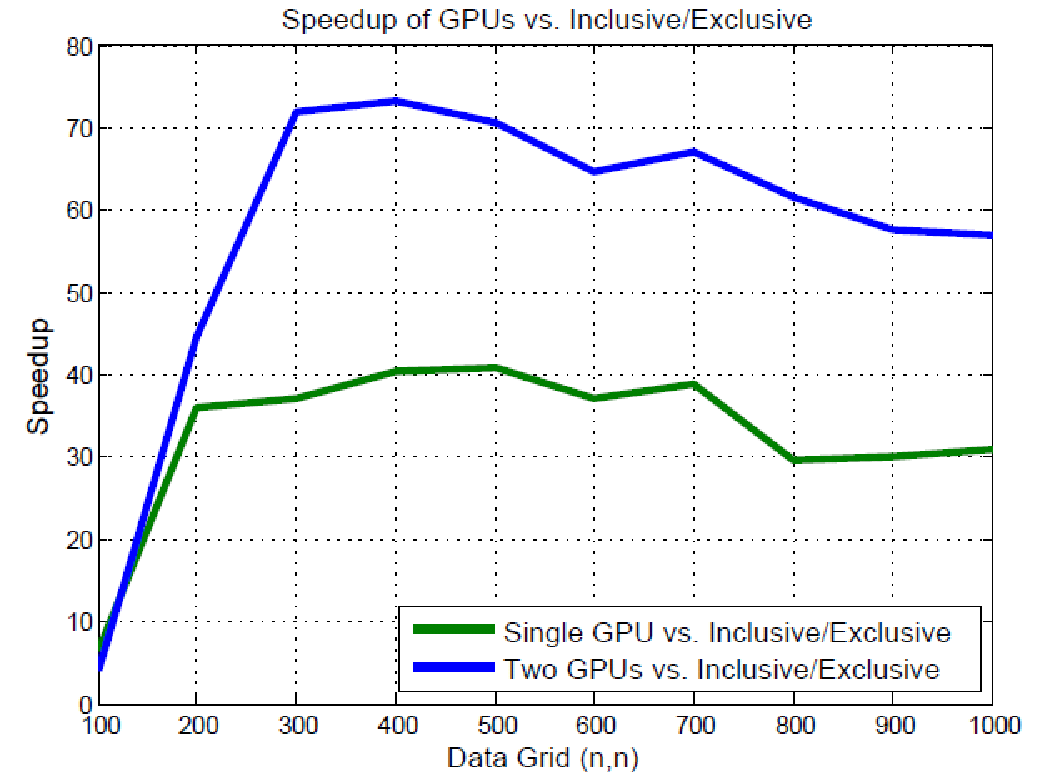
\includegraphics[width=0.8\linewidth]{figtkde/GPUspeedup}
\label{gpu:subfig1}
}\\
~~\subfloat[]{
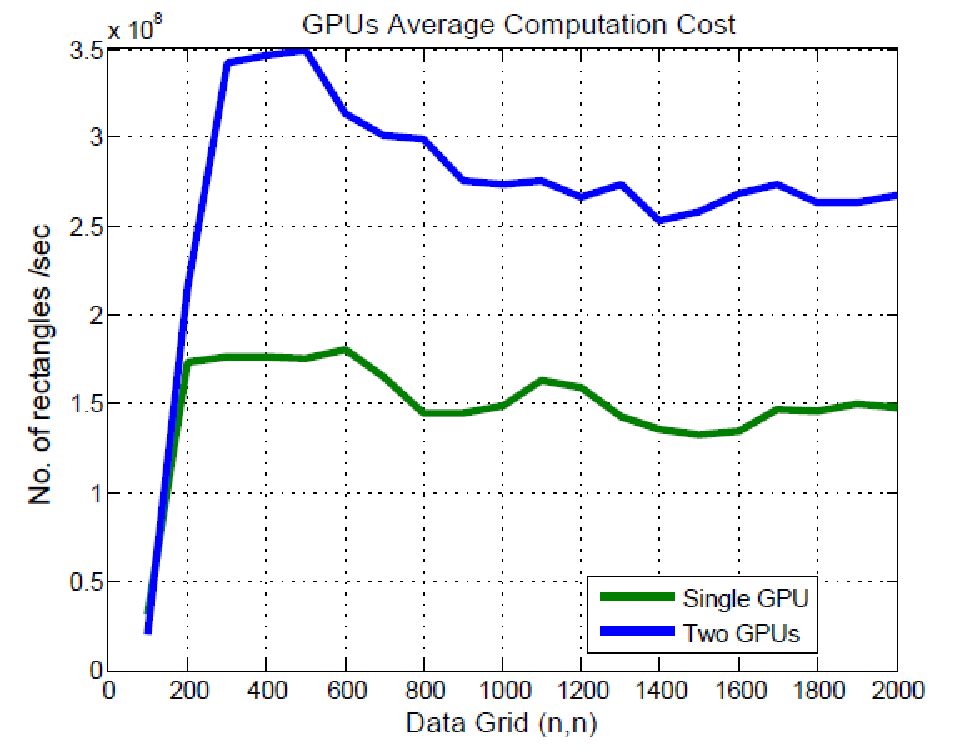
\includegraphics[width=0.8\linewidth]{figtkde/gpurecpersec}
\label{gpu:subfig2}
}
\caption{GPGPUs Cost}\label{gpgpus}
\end{figure}

\begin{figure}[h]
\centering
\subfloat[]{
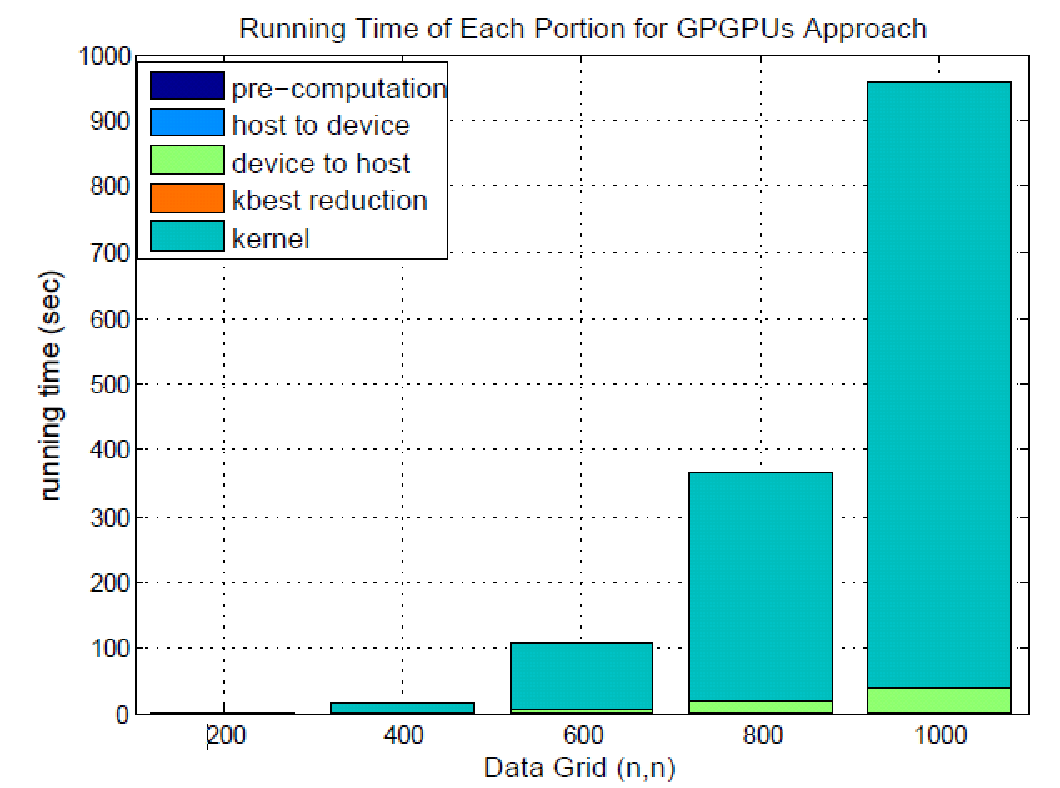
\includegraphics[width=0.9\linewidth]{figtkde/gpuportion}
\label{breakdown:subfig1}
}
\caption{GPGPUs Breakdown parts}\label{breakdown}
\end{figure}

Given the $((((n+1)\times(n+1))/2)^2)$ regions to be searched for a $(n,n)$ grid and the number of threads in each block is $(tx,ty)$. The number of blocks $(bx,by)$ changes the LRT computation performance. In our implementation,each region object takes $8byte$. To fully utilize the shared memory, each block has $(tx,ty)=(16,8)$ threads. We vary the value of $(bx,by)$ for the grids with different size to find the optimal block configuration. To maximize performance:
\begin{itemize}
\item $Max(blocks)\le (bx\times by)\le ((n+1)\times(n+1)/2)^2$, otherwise some blocks won't work.
\item $((n+1)\times(n+1)/2)^2/(bx\times by)\ge (tx\times ty)$ makes each thread processes at least one region.
\item $((n+1)\times(n+1)/2)^2/tx \le (((n+1)\times(n+1))/2))/ty$ is better for reducing bank conflicts since it retrieves more data by rows.
\end{itemize}
If there are too few blocks, each thread processes a quite number of regions and thus performance is degraded. Figure~\ref{optimalgpu} shows the speedup curves using the slowest run for a given grid size as baseline and Table~\ref{tab:op} gives the optimal block configuration. The speedup curves tell us that a speedup of up to two can be achieved by choosing the right block configuration.


\begin{figure}[h]
\centering
{
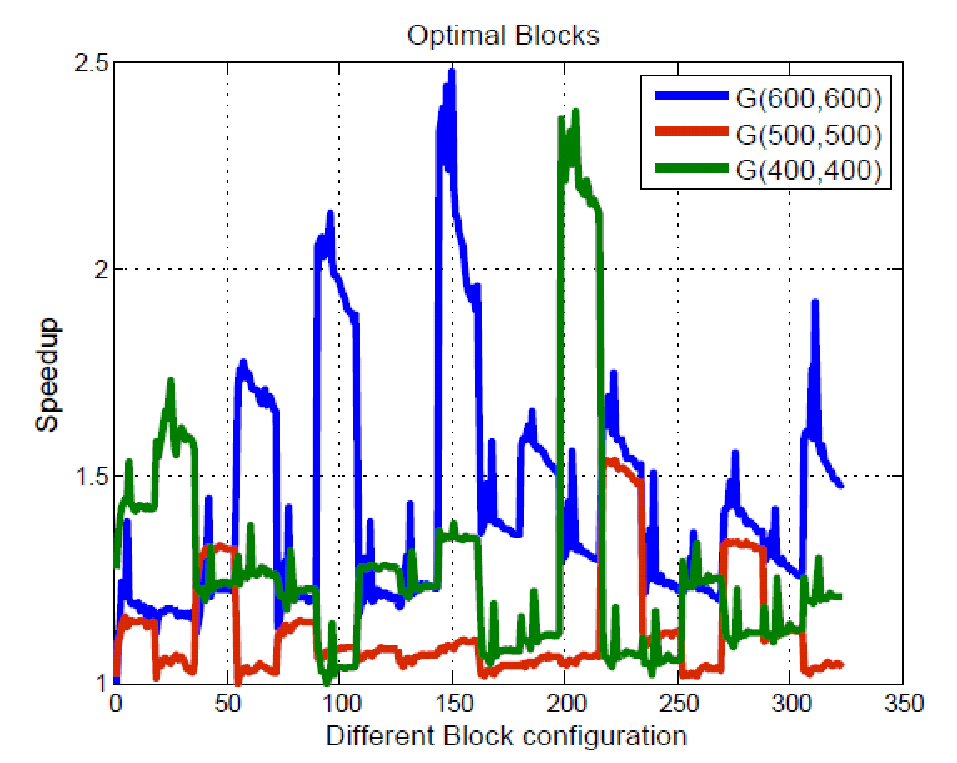
\includegraphics[width=0.8\linewidth]{figtkde/optimalspeed}
\label{optimalgpu:subfig1}
}
\caption{GPGPUs Optimal Blocks Configuration}\label{optimalgpu}
\end{figure}


\begin{table}[t]\small
\centering \caption{Optimized Block Configuration\label{tab:op}} \small
 \begin{tabular}{|c|c|c|}
	\hline
$Grid$ &$block_x$ &$block_y$\\
	\hline
(500,500)     & 128 & 64\\
	\hline
(600,600)     & 192 & 86\\
	\hline
(700,700)     & 176& 86\\
\hline
\end{tabular}
\label{tab:op}
\end{table}

\subsubsection{EC2 Cloud Cluster}
We study a cluster composed of $20 EC2$ high-CPU compute nodes and its effect on MPI application scaling. Instances of this family have proportionally more CPU resources than memory (RAM) and are well suited for compute-intensive applications. Figure~\ref{ec2:subfig1} shows the nearly linear speedup with the increase of number of processes for different grid size on cloud cluster. The computation speed of rectangles is plotted out in Figure~\ref{ec2:subfig2}, it shows the computation speed is faster with the increase number of processes on a given data grid and also verifies the constant computation speed for different data grid by a given number of processes.


\begin{figure}[h]
\centering
\subfloat[]{
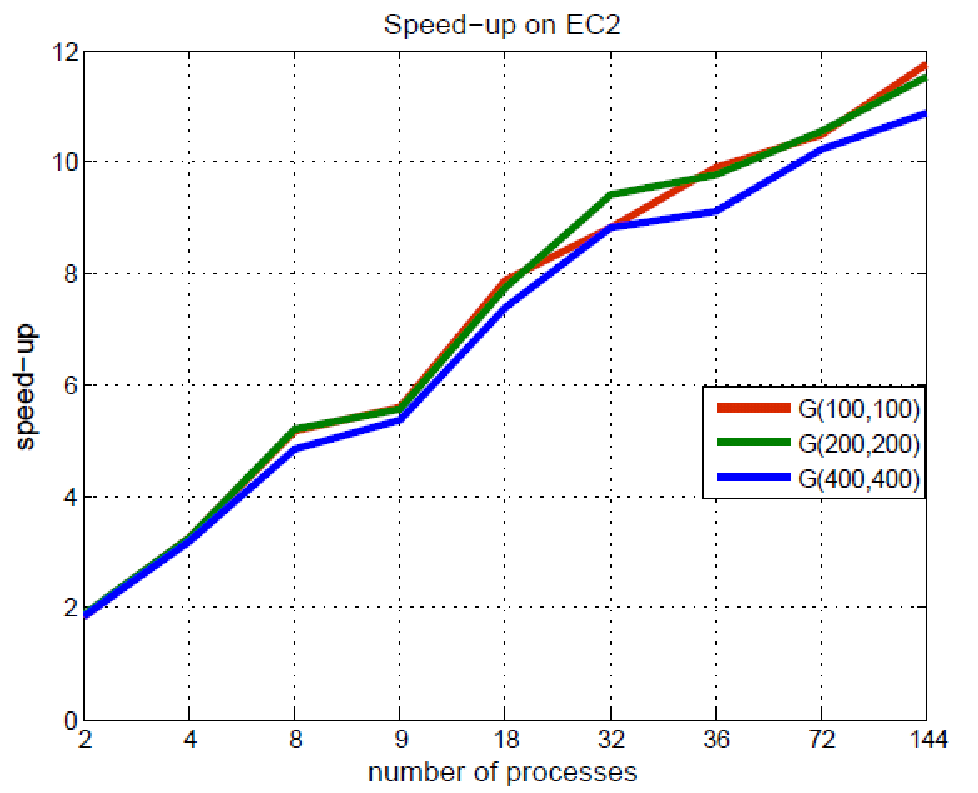
\includegraphics[width=0.85\linewidth]{figtkde/ec2speedup}
\label{ec2:subfig1}
}\\
~~\subfloat[]{
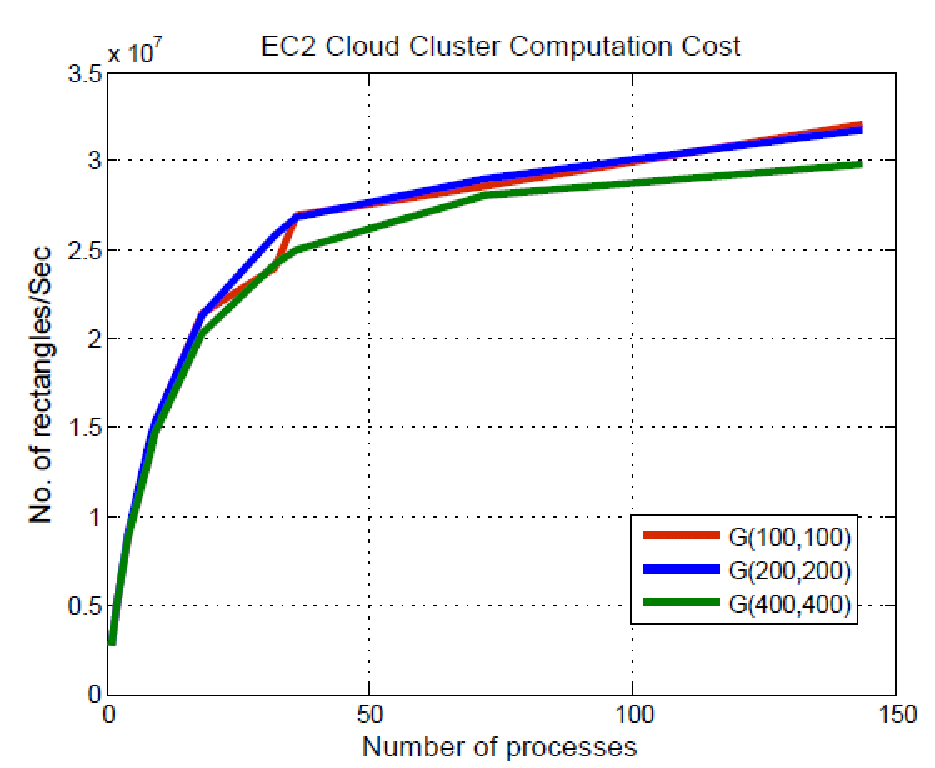
\includegraphics[width=0.85\linewidth]{figtkde/ec2compcost}
\label{ec2:subfig2}
}
\caption{Speed-up of LRT computation on EC2 cloud cluster }\label{ec2}
\end{figure}

\subsection{Discussion}
From the above results, we further analyze of LRT computation on different architectures. Table~\ref{cmtable} shows the related factors to the LRT performance on different architectures, the speedup and processing speed of rectangles from these factors. We plot the number of rectangles processed per second for data grid $(1000,1000)$ on the following different architectures: multi-core, GPGPU and EC2 cloud cluster. The results are shown in Figure~\ref{cm}. The dashed line in the figure is the processing speed of Inclusive/Exclusive approach on single CPU. From the figure, we can see that the GPGPU approach performs much better than multi-core and EC2, which is almost one order of magnitude faster. As the number of cores and the number of processes increase, the LRT processing speed is improved. \\

\begin{comment}
\begin{table*}[t]
\begin{tabular}{|l|l|l|l|} \hline
\multicolumn{4}{|c|}{Different Parallel Architectures} \\
\hline
\multirow{1}{*}{}   & Multi-core & GPGPUs & EC2 Cluster  \\
 \hline
\multirow{1}{*}{Factors}   & $(n,nc)$  & $(n,ng,nb)$  & $(n,np)$ \\
 \hline
\multirow{2}{*}{SpeedUp} & (1) linear to $nc$ for a given $n$& (1) almost linear to $ng$ for given $n$ and $nb$ &  (1)linear to $np$ for a given $n$ \\
{} & {}& (2) constant to different $n$ for given ng and nb& {} \\
{} & {}& (3) $\times$(1.5~2.5) by choosing an optimal nb for given $n$ and $ng$ &{}\\
 \hline
 \multirow{2}{*}{$no_r$/sec} & (1) linear to $nc$ for a given $n$&(1)almost constant for a given $n$& \\
 \multirow{2}{*}{} & {}&(2)almost linear to $ng$ for a given $n$& (1)is proportional to $\log (np)$\\
 \hline
\end{tabular}
 \caption{The comparison of different parallel implementations to Inclusive/Exclusive sequential implementation. Note: $n$ is grid size, $nc$ is the number of cores, $ng$ is the number of GPGPUs, $nb$ is the block number for GPGPU kernel and $np$ is the number of processes. }\label{cmtable}
\end{table*}
\end{comment}

\begin{figure}[h]
\centering
\subfloat[]{
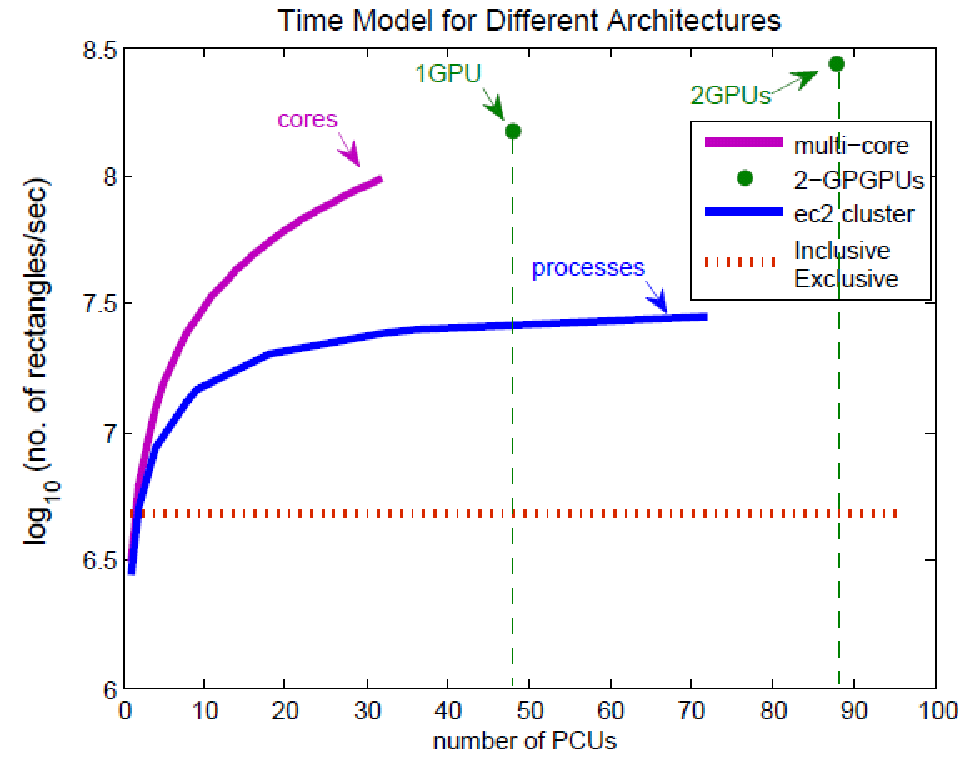
\includegraphics[width=0.85\linewidth]{figtkde/combined}
\label{cm}
}
\caption{Time Model of Different Architectures}\label{cm}
\end{figure}

\section {Related Work} \label{RW}
Previous attempts to parallelize LRT computation have only achieved limited success. For example, the Spatial Scan Statistic (SSS), which
is a special case of LRT for Poisson data, is available
as a program under the name SatScan~\cite{sat}. It has been parallelized for multi-core CPU environments and its extension for a GPGPU hardware~\cite{Larew} has
achieved improved speed up of two over the multi-core
baseline. The GPGPU implementation in~\cite{Larew} has proposed loading parts
of the data into shared memory but has achieved only a modest speed up. The
other attempt of~\cite{zhao} applied their own implementation of a spatial
scan statistic program on the GPU to the epidemic disease dataset. This solution is only applicable to its special disease scenario.
In each of these cases, we believe there is further room for optimising the
algorithms for the parallel architectures by devising the fine-grained parallelism strategies.

Furthermore, all the existing parallel solutions perform
LRT tests in a circular or cylindrical way, not in a grid-based scenario. Our parallel
solution is different and provides a fully paralleled template for
1EXP-LRT computation in a grid.

\section{Conclusion}\label{CC}
The Likelihood Ratio Test Statistic (LRT) is a state-of-the-art method for identifying hotspots or anomalous
regions in large spatial settings. To speed up the LRT computation for 1EXP family, this paper proposed three ideas: (i) a novel range mapping scheme is proposed to fully enumerate all the regions in a contiguous space. (ii) a dynamic pre-computation algorithm is implemented to reduce the cost of aggregating intermediate statistics. (iii) to save space and improve processing speed, kbest reduction scheme is presented to accumulate distributed results. We did the implementations on different parallel architectures: Multi-core, Multi-GPGPU and EC2 cloud cluster and extensive experiments are done correspondingly. From the results, we see that pre-computation approach has a linear speed-up with the data grid size comparing to the brute-force sequential approach. Then we compare the speed-up on different parallel architectures using pre-computation approach as baseline. The speed-up of these parallel approach increases near-linearly with the increase of the number of ``parallel
computing unit'' on different architectures. In concert, the parallel approaches yield a speed up of nearly four thousand times compared to
their sequential counterpart. Further analysis on the processing speed of number of rectangles is given. This provides some recommended information for choosing the right architectures on various factors. Moving the computation of the LRT statistics to the parallel architectures enables the use of this sophisticated method of outlier detection for larger
spatial grids than previously reported.

In future, we will apply the range mapping scheme on non-1EXP family distribution using pruning strategy~\cite{jour}. A unified parallel approach will be provided for generalized LRT computation in spatial grids.

\appendices

\section{Inclusive/Exclusive Statistics Aggregation }

\begin{equation}
\begin{split}
|R(x_1,y_1,x_2,y_2)|& = |A(x_2,y_2)| + |B(x_1,y_1)| + |X(x_1,y_2)| \\& \quad + |Y(x_2,y_1)| - |G|
\end{split}
\end{equation}

\begin{proof}
\begin{equation}
\begin{split}
|R|&=\sum_{i=1}^{x_2}\sum_{j=1}^{y_2}c_{i,j}+\sum_{i={x_1}}^{n}\sum_{j={y_1}}^{n}c_{i,j}+\sum_{i={x_2}}^{n}\sum_{j=1}^{y_1}c_{i,j}+\sum_{i=1}^{x_1}\sum_{j={y_2}}^{n}c_{i,j}\\& \quad-\sum_{i=1}^{n}\sum_{j=1}^{n}c_{i,j}\\&\quad=\sum_{i=1}^{x_1}\sum_{j=1}^{y_2}c_{i,j}+\sum_{i={x_1}}^{x_2}(\sum_{j=1}^{y_1}c_{i,j}+\sum_{j={y_1}}^{y_2}c_{i,j})+\sum_{i={x_1}}^{n}\sum_{j={y_1}}^{n}c_{i,j}\\& \quad +\sum_{i={x_2}}^{n}\sum_{j=1}^{y_1}c_{i,j}+\sum_{i=1}^{x_1}\sum_{j={y_2}}^{n}c_{i,j}\\&\quad=\sum_{i=1}^{x_1}\sum_{j=1}^{n}c_{i,j}+\sum_{i={x_1}}^{x_2}\sum_{j=1}^{y_1}c_{i,j}+|R|+|R|+\sum_{i={x_1}}^{x_2}\sum_{j={y_2}}^{n}c_{i,j}\\&\quad+\sum_{i={x_2}}^n\sum_{j=1}^{n}c_{i,j}-\sum_{i=1}^n\sum_{j=1}^{n}c_{i,j}
\\&\quad =\sum_{i=1}^n\sum_{j=1}^{n}c_{i,j}+|R|-\sum_{i=1}^n\sum_{j=1}^{n}c_{i,j}\\&\quad =|R|
\end{split}
\end{equation}
\end{proof}

\begin{definition}
\begin{equation}
A(i,j)=\sum_{k=1}^{i}\sum_{l=1}^{j}c_{i,j}\mbox{\quad for all $1\leq i,j\leq n$}.
\end{equation}
\end{definition}

\begin{lemma}
\begin{equation}
A(i,j)=A_{i-1,j}+A_{i,j-1}-A_{i-1,j-1}+c_{i,j} \mbox{\quad for all $1<i,j\leq n$}.
\end{equation}
\end{lemma}

\begin{proof}
\begin{eqnarray*}
A(i,j)& = & \sum_{k=1}^{i-1}\sum_{l=1}^{j}c_{k,l}+a_{i,j-1}-a_{i-1,j-1}+c_{i,j}\\
 & = & \sum_{k=1}^{i-1}\left(\sum_{l=1}^{j-1}c_{k,l}+c_{k,j}\right)+a_{i,j-1}-\sum_{k=1}^{i-1}\sum_{l=1}^{j-1}c_{k,l}+c_{i,j}\\
 & = & \sum_{k=1}^{i-1}c_{k,j}+c_{i,j}+a_{i,j-1}\\
 & = & \sum_{k=1}^{i}c_{k,j}+a_{i,j-1}\\
 & = & \sum_{k=1}^{i}c_{k,j}+\sum_{k=1}^{i}\sum_{l=1}^{j-1}c_{k,l}\\
 & = & A(i,j)
\end{eqnarray*}

\end{proof}

\begin{definition}
\begin{equation}
X_{i,j}=\sum_{k=i}^{n}\sum_{l=1}^{j}c_{i,j}\mbox{\quad for all $1\leq i,j\leq n$}.
\end{equation}
\end{definition}

\begin{lemma}
\begin{equation}
X_{i,j}=X_{i,j-1}+X_{i+1,j}-X_{i+1,j-1}+c_{i,j} \mbox{\quad for all $1<i,j\leq n$}.
\end{equation}
\end{lemma}

\begin{proof}
\begin{eqnarray*}
X_{i,j}& = & \sum_{k=i+1}^{n}\sum_{l=1}^{j}c_{k,l}+X_{i,j-1}-X_{i+1,j-1}+c_{i,j}\\
 & = & \sum_{k=i+1}^{n}\left(\sum_{l=1}^{j-1}c_{k,l}+c_{k,j}\right)+X_{i,j-1}-\sum_{k=1+1}^{n}\sum_{l=1}^{j-1}c_{k,l}+c_{i,j}\\
 & = & \sum_{k=i+1}^{n}c_{k,j}+c_{i,j}+X_{i,j-1}\\
 & = & \sum_{k=i}^{n}c_{k,j}+X_{i,j-1}\\
 & = & \sum_{k=i}^{n}c_{k,j}+\sum_{k=i}^{n}\sum_{l=1}^{j-1}c_{k,l}\\
 & = & X_{i,j}
\end{eqnarray*}
\end{proof}

\begin{definition}
\begin{equation}
X_{i,j}=\sum_{k=i}^{n}\sum_{l=1}^{j}c_{i,j}\mbox{\quad for all $1\leq i,j\leq n$}.
\end{equation}
\end{definition}

\begin{lemma}
\begin{equation}
X_{i,j}=X_{i,j-1}+X_{i+1,j}-X_{i+1,j-1}+c_{i,j} \mbox{\quad for all $1<i,j\leq n$}.
\end{equation}
\end{lemma}

\begin{proof}
\begin{eqnarray*}
X_{i,j}& = & \sum_{k=i+1}^{n}\sum_{l=1}^{j}c_{k,l}+X_{i,j-1}-X_{i+1,j-1}+c_{i,j}\\
 & = & \sum_{k=i+1}^{n}\left(\sum_{l=1}^{j-1}c_{k,l}+c_{k,j}\right)+X_{i,j-1}-\sum_{k=1+1}^{n}\sum_{l=1}^{j-1}c_{k,l}+c_{i,j}\\
 & = & \sum_{k=i+1}^{n}c_{k,j}+c_{i,j}+X_{i,j-1}\\
 & = & \sum_{k=i}^{n}c_{k,j}+X_{i,j-1}\\
 & = & \sum_{k=i}^{n}c_{k,j}+\sum_{k=i}^{n}\sum_{l=1}^{j-1}c_{k,l}\\
 & = & X_{i,j}
\end{eqnarray*}
\end{proof}

\begin{definition}
\begin{equation}
y_{i,j}=\sum_{k=1}^{i}\sum_{l=j}^{n}c_{i,j}\mbox{\quad for all $1\leq i,j\leq n$}.
\end{equation}
\end{definition}

\begin{lemma}
\begin{equation}
Y_{i,j}=Y_{i-1,j}+Y_{i,j+1}-Y_{i-1,j+1}+c_{i,j} \mbox{\quad for all $1<i,j\leq n$}.
\end{equation}
\end{lemma}

\begin{proof}
\begin{eqnarray*}
Y_{i,j}& = & \sum_{k=1}^{i-1}\sum_{l=j}^{n}c_{k,l}+Y_{i,j+1}-Y_{i-1,j+1}+c_{i,j}\\
 & = & \sum_{k=1}^{i-1}\left(\sum_{l=j+1}^{n}c_{k,l}+c_{k,j}\right)+Y_{i,j+1}-\sum_{k=1}^{i-1}\sum_{l=j+1}^{n}c_{k,l}+c_{i,j}\\
 & = & \sum_{k=1}^{i-1}c_{k,j}+c_{i,j}+Y_{i,j+1}\\
 & = & \sum_{k=1}^{i}c_{k,j}+Y_{i,j+1}\\
 & = & \sum_{k=1}^{i}c_{k,j}+\sum_{k=1}^{i}\sum_{l=j+1}^{n}c_{k,l}\\
 & = & Y_{i,j}
\end{eqnarray*}
\end{proof}

\section{Pre-processing of Inclusive/Exclusive Computation}

\begin{algorithm}[t!]\small
\label{pre1}
\caption{Inclusive/Exclusive Pre-computation for Set B}\label{pre1}
Input: data grid (G) \\
Output: accumulated counts $B(i,j)$\\
------------------------------------------------------------------ \\
\begin{algorithmic}[1]
\STATE //Initialize first element $B(n-1,n-1)$
\STATE {\textit { $B(n-1,n-1)$\(\leftarrow\)$G(n-1,n-1)$}}
\STATE //accumulation of remaining elements in last column
\FOR{\textit  j\(\leftarrow\)(n-1) to \textit{1}}
\STATE{\textit { $B(j-1,n-1)$ \(\leftarrow\) $G(i-1,n-1)$ +$B(j,n-1)$}}
\ENDFOR
\STATE //accumulation of remaining elements in last row
\FOR{\textit  i\(\leftarrow\)(n-1) to \textit{1}}
\STATE  {\textit {$B(n-1,i-1)$\(\leftarrow\)$G(n-1,i-1)$ + $B(n-1,i)$}}
\ENDFOR
\STATE //accumulation of all the elements in remaining rows and columns
\FOR{\textit  k\(\leftarrow\)1 to \textit{n}}
\FOR{\textit  i\(\leftarrow\)(n-1) to \textit{k}}
\STATE  {\textit B(i-k,n-1-k)\(\leftarrow\) G(i-k,n-1-k)+B(i-k+1,n-1-k)+B(i-k,n-k)-B(i-k+1,n-k)}
\ENDFOR
\FOR{\textit  j\(\leftarrow\)(n-1) to \textit{k}}
\STATE  {\textit B(n-1-k,j-k)\(\leftarrow\)G(n-1-k,j-k)+B(n-1-k,j-k+1)+ B(n-k,j-k)-B(n-k,j-k+1)}
\ENDFOR
\ENDFOR
\end{algorithmic}
\end{algorithm}

\begin{algorithm}[t!]\small
\label{pre2}
\caption{Pre-processing of Inclusive/Exclusive Computation for Set X}\label{pre2}
------------------------------------------------------------------ \\
\begin{algorithmic}[1]
\STATE //Initialize first column
\FOR{\textit  i\(\leftarrow\)1 to \textit{n}}
\STATE {\textit {X(i,0)\(\leftarrow\)0 }}
\ENDFOR
\STATE //Initialize last row
\FOR{\textit  j\(\leftarrow\)1 to \textit{n}}
\STATE  {\textit { X(n-1,j)\(\leftarrow\)0 }}
\ENDFOR
\STATE //Iterate over all diagonal elements
\FOR{\textit  k\(\leftarrow\)1 to \textit{n}}
\STATE //associate columns of diagonal elements
\FOR{\textit  i\(\leftarrow\)n-1 to \textit k}
\STATE  {\textit X(i-k,k)\(\leftarrow\)G(i-k+1,k-1)+X(i-k+1,k)+X(i-k,k-1)-X(i-k+1,k-1)}
\ENDFOR
\STATE // associate columns of diagonal element k
\FOR{\textit j\(\leftarrow\)k to \textit{n}}
\STATE  {\textit X(n-1-k,j)\(\leftarrow\)G(n-k,j-1)+X(n-1-k,j-1)+X(n-k,j)-X(n-k,j-1)}
\ENDFOR
\ENDFOR
\end{algorithmic}
\end{algorithm}

\begin{algorithm}[t!]\small
\label{pre1}
\caption{Inclusive/Exclusive Pre-computation for Set Y}\label{pre1}
Input: data grid (G) \\
Output: accumulated counts $Y(i,j)$\\
------------------------------------------------------------------ \\
\begin{algorithmic}[1]
\STATE //Initialize last column
\FOR{\textit  i\(\leftarrow\)1 to \textit{n}}
\STATE {\textit {Y(i,n-1)\(\leftarrow\)0 }}
\ENDFOR
\STATE //Initialize first row
\FOR{\textit  j\(\leftarrow\)1 to \textit{n}}
\STATE  {\textit { Y(0,j)\(\leftarrow\)0 }}
\ENDFOR
\STATE //Iterate over all diagonal elements
\FOR{\textit  k\(\leftarrow\)1 to \textit{n}}
\STATE //associate columns of diagonal elements
\FOR{\textit  i\(\leftarrow\)k to \textit (n-1)}
\STATE  {\textit Y(i,n-1-k)\(\leftarrow\)G(i-1,n-k)+Y(i-1,n-1-k)+ Y(i,n-k)-Y(i-1,n-k)}
\ENDFOR
\STATE // associate columns of diagonal element k
\FOR{\textit j\(\leftarrow\)(n-1) to \textit{k}}
\STATE  {\textit Y(k,n-k)\(\leftarrow\)G(k-1,n-k+1)+Y(k,n-k+1)+Y(k-1,n-k)-Y(k-1,n-k+1)}
\ENDFOR
\ENDFOR
\end{algorithmic}
\end{algorithm}



% references section

% can use a bibliography generated by BibTeX as a .bbl file
% BibTeX documentation can be easily obtained at:
% http://www.ctan.org/tex-archive/biblio/bibtex/contrib/doc/
% The IEEEtran BibTeX style support page is at:
% http://www.michaelshell.org/tex/ieeetran/bibtex/
\bibliographystyle{IEEEtran}
\bibliography{gpulrt}
% argument is your BibTeX string definitions and bibliography database(s)
%\bibliography{IEEEabrv,../bib/paper}
%
% <OR> manually copy in the resultant .bbl file
% set second argument of \begin to the number of references
% (used to reserve space for the reference number labels box)

%\begin{thebibliography}{1}

%\bibitem{IEEEhowto:kopka}
%This is an example of a book reference
%H. Kopka and P.W. Daly, \emph{A Guide to {\LaTeX}}, third ed. Harlow, U.K.: Addison-Wesley, 1999.


%This is an example of a Transactions article reference
%D.S. Coming and O.G. Staadt, "Velocity-Aligned Discrete Oriented Polytopes for Dynamic Collision Detection," IEEE Trans. Visualization and Computer Graphics, vol.�14,� no.�1,� pp. 1-12,� Jan/Feb� 2008, doi:10.1109/TVCG.2007.70405.

%This is an example of a article from a conference proceeding
%H. Goto, Y. Hasegawa, and M. Tanaka, "Efficient Scheduling Focusing on the Duality of MPL Representation," Proc. IEEE Symp. Computational Intelligence in Scheduling (SCIS '07), pp. 57-64, Apr. 2007, doi:10.1109/SCIS.2007.367670.

%This is an example of a PrePrint reference
%J.M.P. Martinez, R.B. Llavori, M.J.A. Cabo, and T.B. Pedersen, "Integrating Data Warehouses with Web Data: A Survey," IEEE Trans. Knowledge and Data Eng., preprint, 21 Dec. 2007, doi:10.1109/TKDE.2007.190746.

%Again, see the IEEEtrans_HOWTO.pdf for several more bibliographical examples. Also, more style examples
%can be seen at http://www.computer.org/author/style/transref.htm
%\end{thebibliography}

% biography section
%
% If you have an EPS/PDF photo (graphicx package needed) extra braces are
% needed around the contents of the optional argument to biography to prevent
% the LaTeX parser from getting confused when it sees the complicated
% \includegraphics command within an optional argument. (You could create
% your own custom macro containing the \includegraphics command to make things
% simpler here.)
%\begin{biography}[{\includegraphics[width=1in,height=1.25in,clip,keepaspectratio]{mshell}}]{Michael Shell}
% or if you just want to reserve a space for a photo:

% insert where needed to balance the two columns on the last page with
% biographies
%\newpage


% You can push biographies down or up by placing
% a \vfill before or after them. The appropriate
% use of \vfill depends on what kind of text is
% on the last page and whether or not the columns
% are being equalized.

%\vfill

% Can be used to pull up biographies so that the bottom of the last one
% is flush with the other column.
%\enlargethispage{-5in}



% that's all folks
\end{document}



